% Sherman v1
\chapter{Student Handouts}

Paper handouts were used in three of the activities to provide instructions and work space for the students. They are included here.

%I can also make these not full-page %by using the includegraphics instead of includepdf
%if that is better. It would allow for captions like normal images or the insert to be on the same page as its title.

%\section{Gear Reduction Handout}
	\label{sec:gearshandout}
	
	Figures \ref{fig:gearshandout1} and \ref{fig:gearshandout2} show the handout that was provided to students when doing the Gear Reduction activity. At the conclusion of the session the students were asked to draw their design in the style of the example in Figure \ref{fig:gearshandout2}.
	
	%TODO replace these ugly images with actual scans
	
	\begin{figure}
	\centering
	%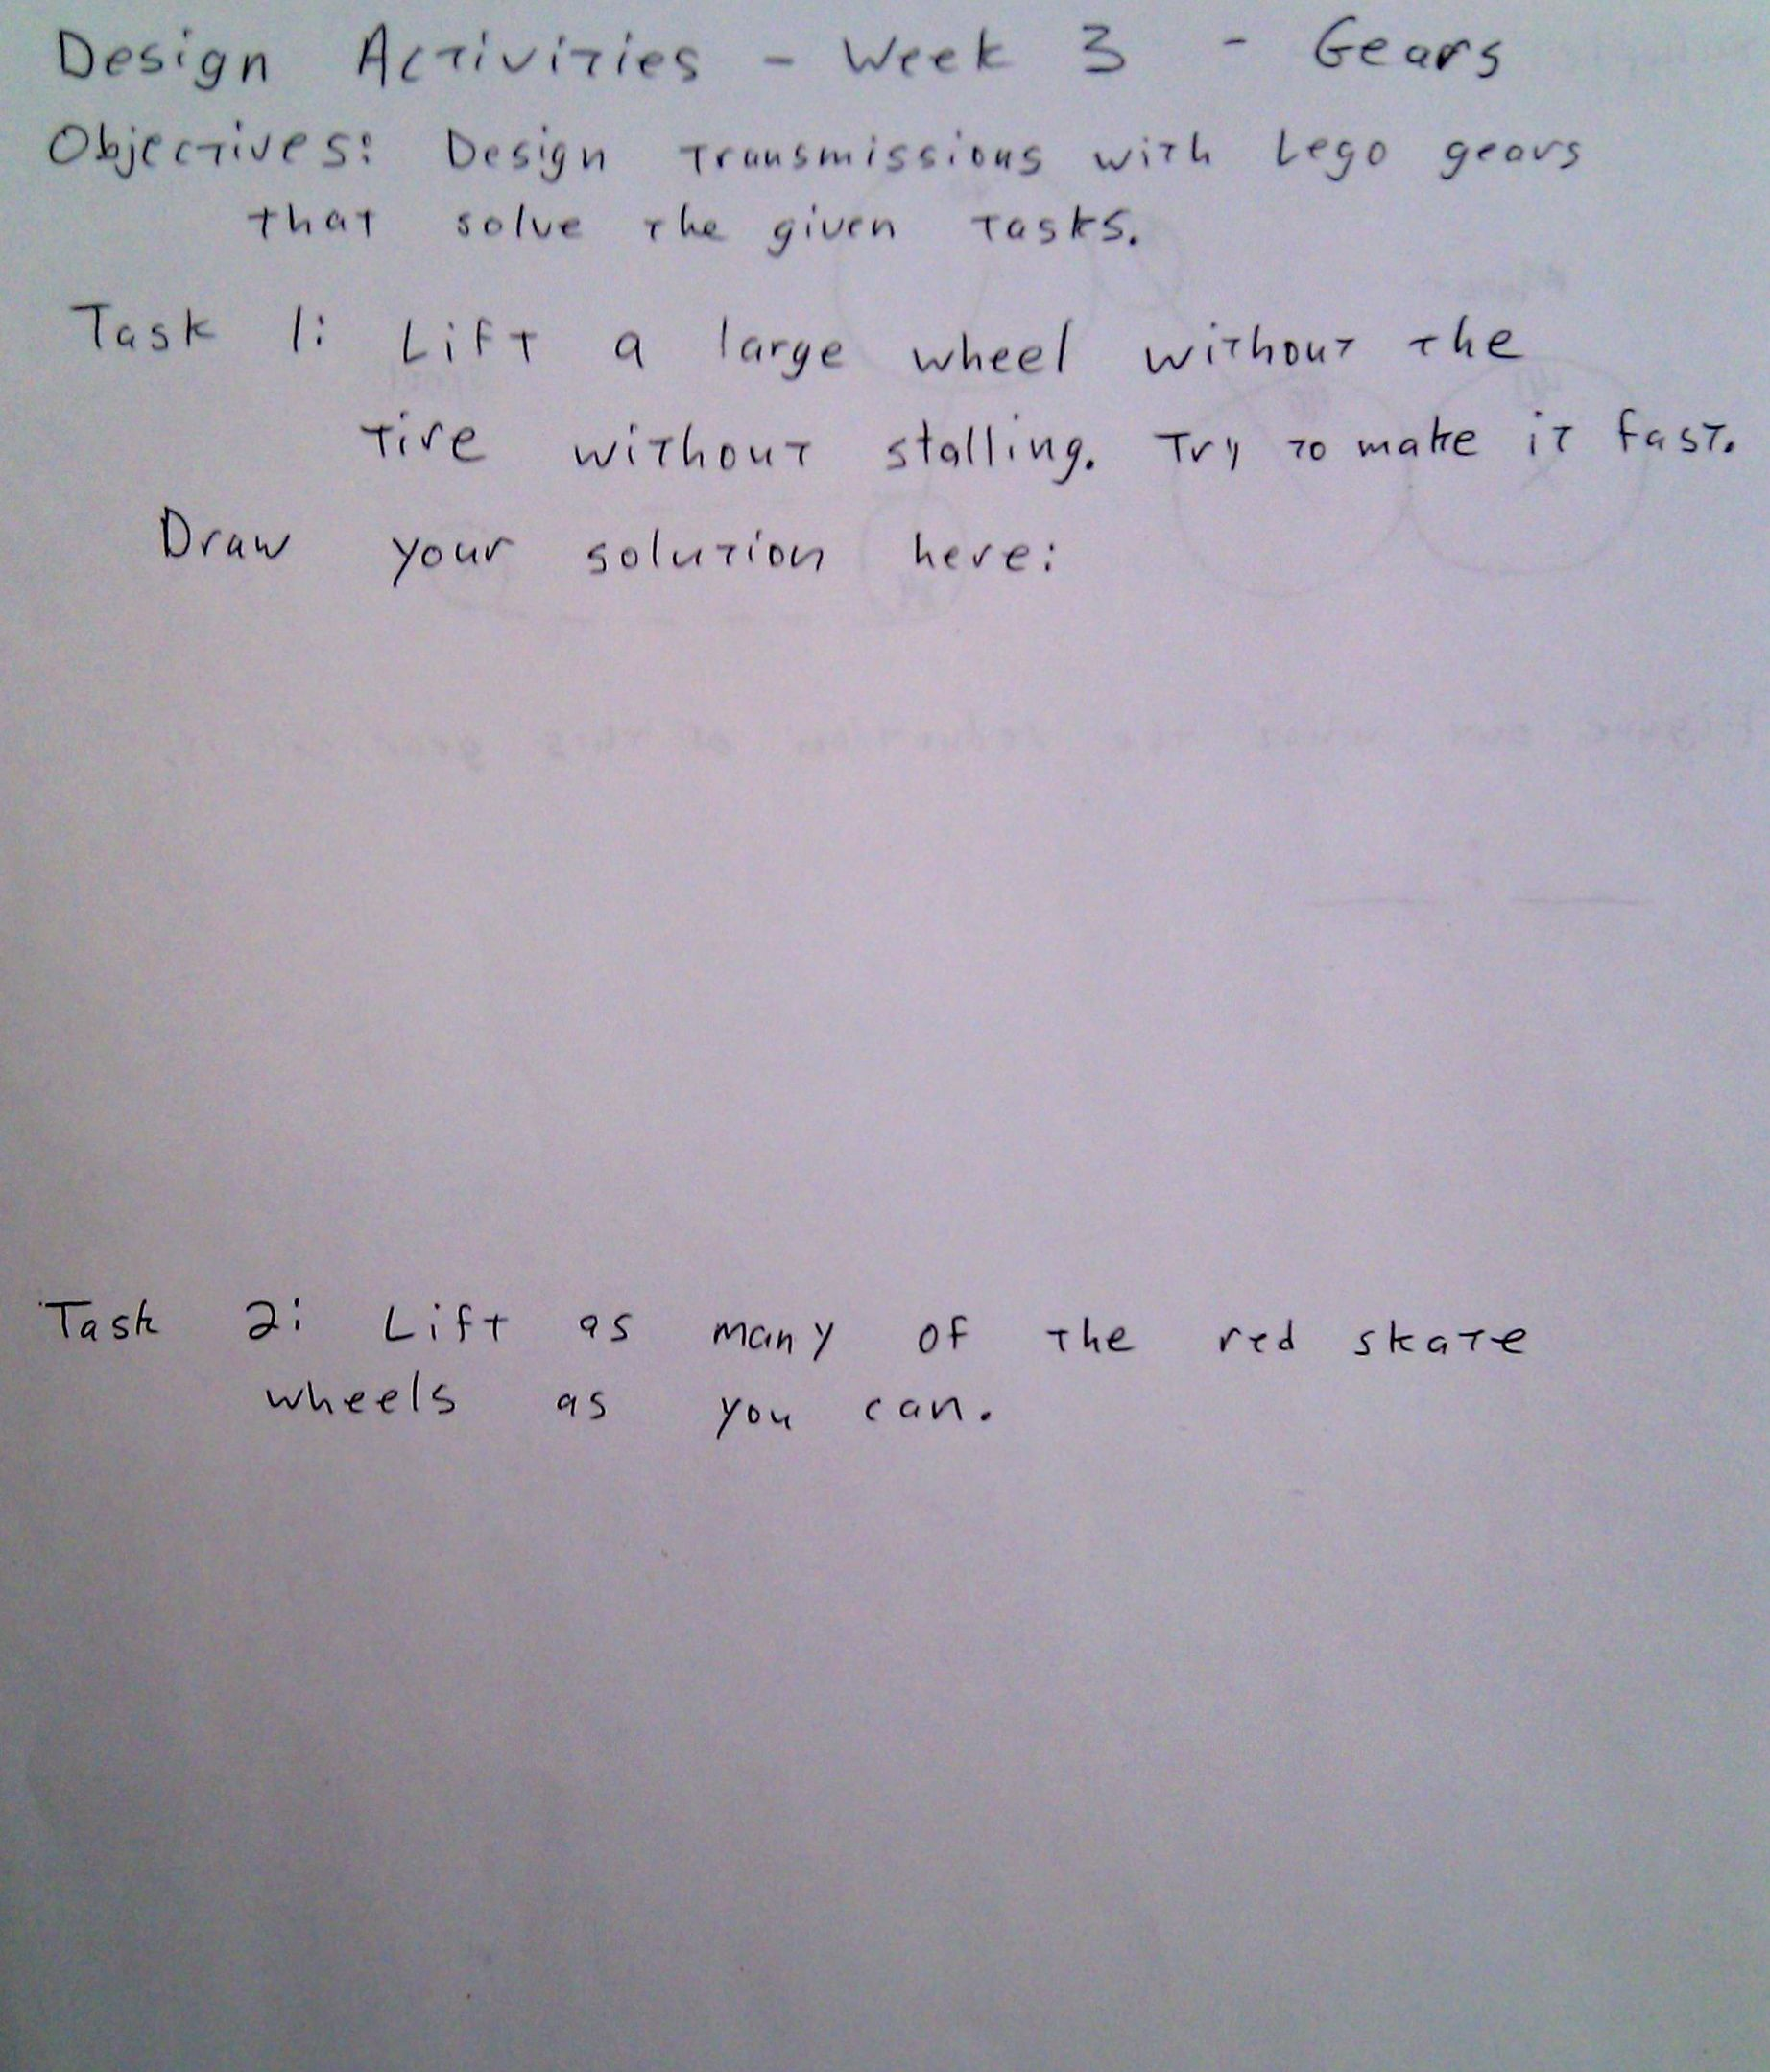
\includegraphics[width=\textwidth]{appendix/gear-handout-1}
	\caption{First page of the worksheet given to students during the Gear Reduction activity.}
	\label{fig:gearshandout1}
	\end{figure}

	\begin{figure}
	\centering
	%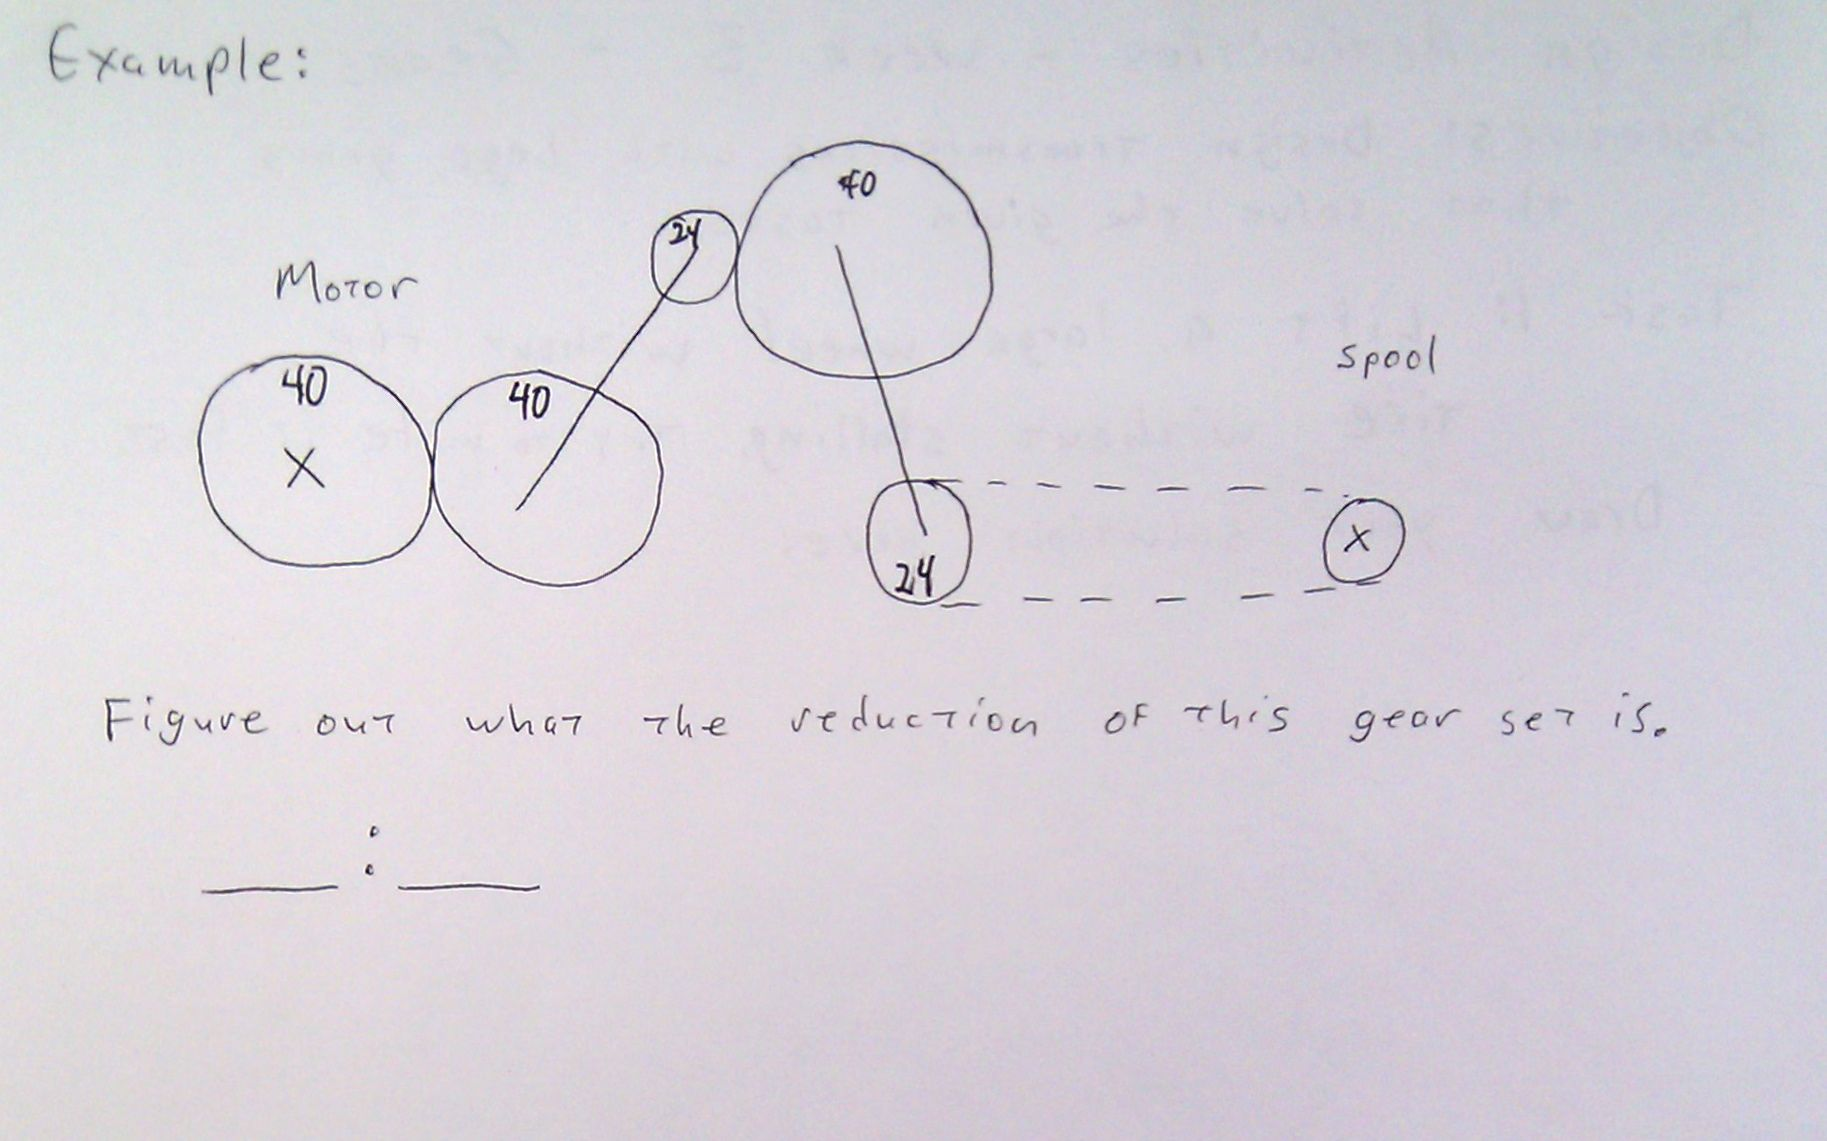
\includegraphics[width=\textwidth]{appendix/gear-handout-2}
	\caption{Second page of the worksheet given to students during the Gear Reduction activity.}
	\label{fig:gearshandout2}
	\end{figure}

%\section{Word Search Handout}
	\label{sec:wordsearchhandout}
	Figures \ref{fig:StudentWorksheet1} through \ref{fig:StudentWorksheet3} show the handout that was provided to students when during the Word Search activity.
	
	%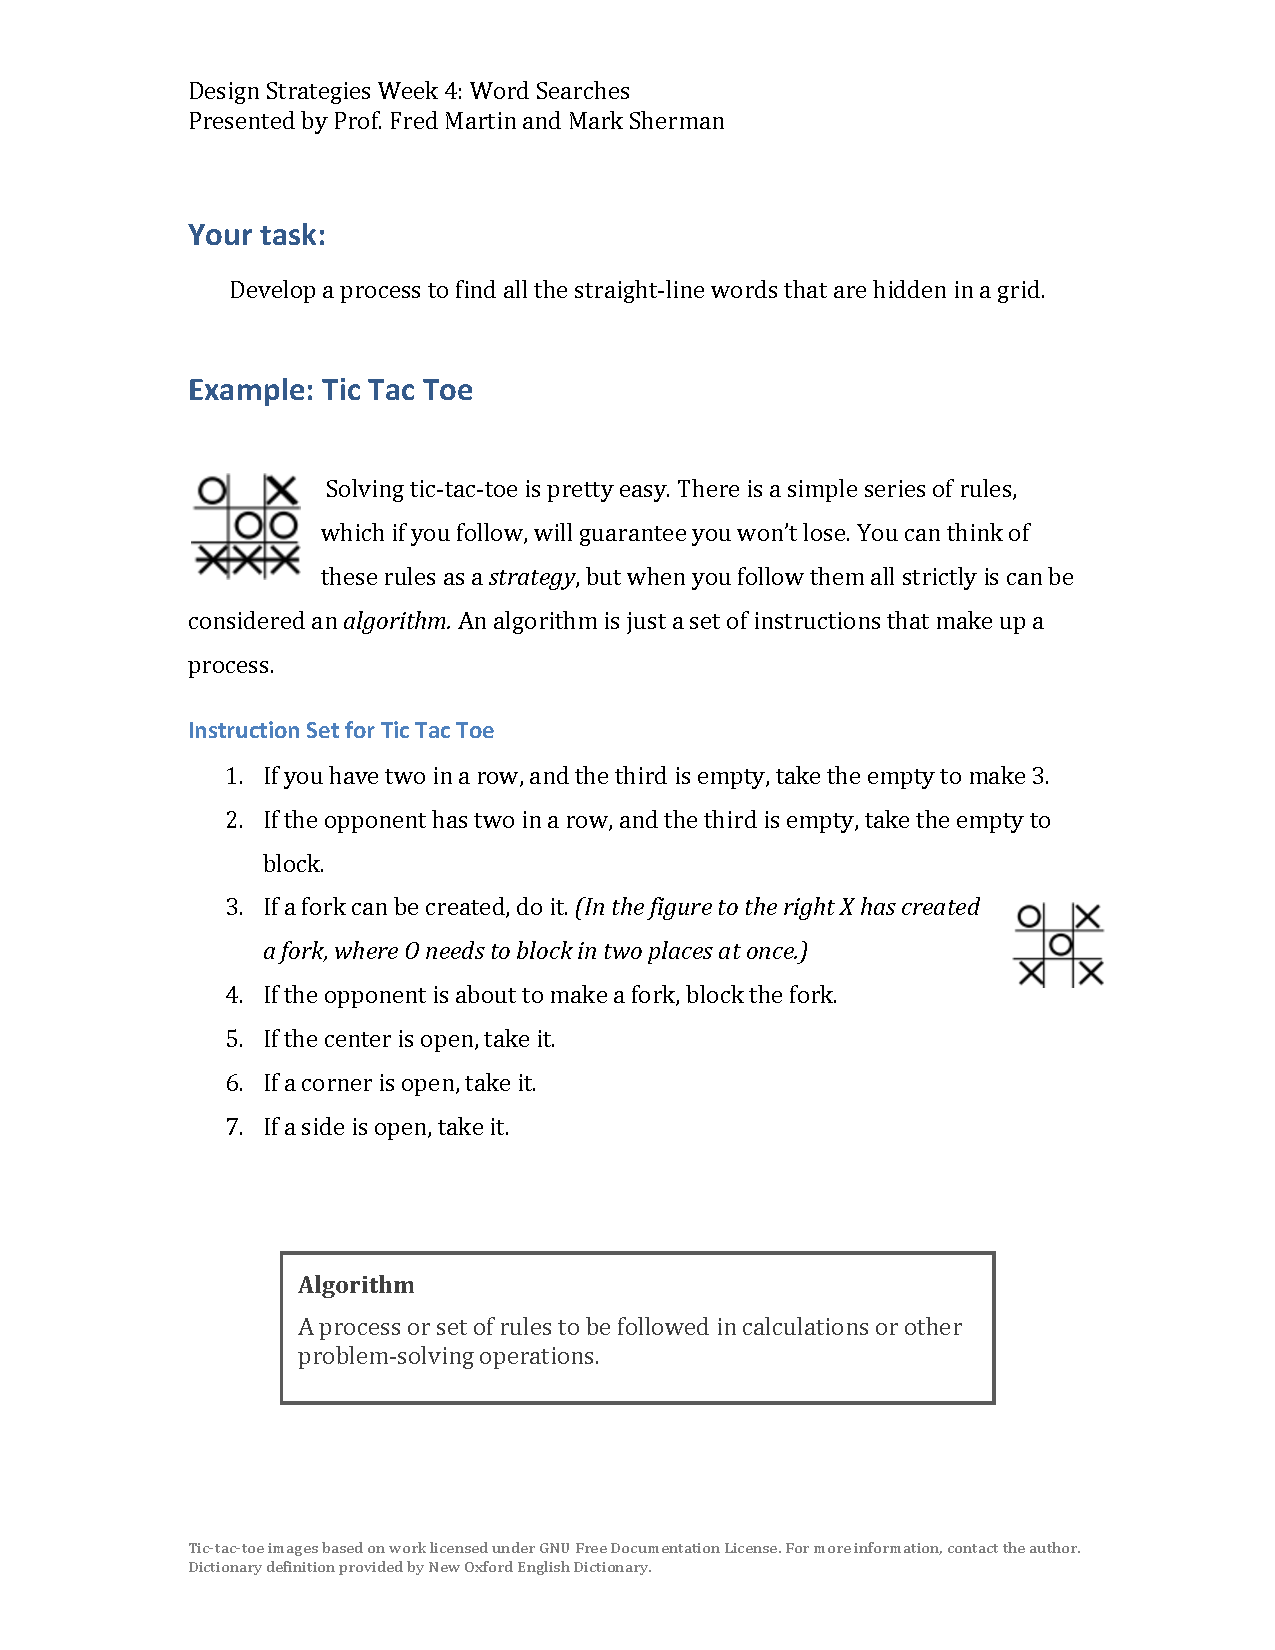
\includepdf[pages=-]{appendix/word_search_worksheet.pdf}

\begin{figure}%  figure placement: here, top, bottom, or page
   \centering
   %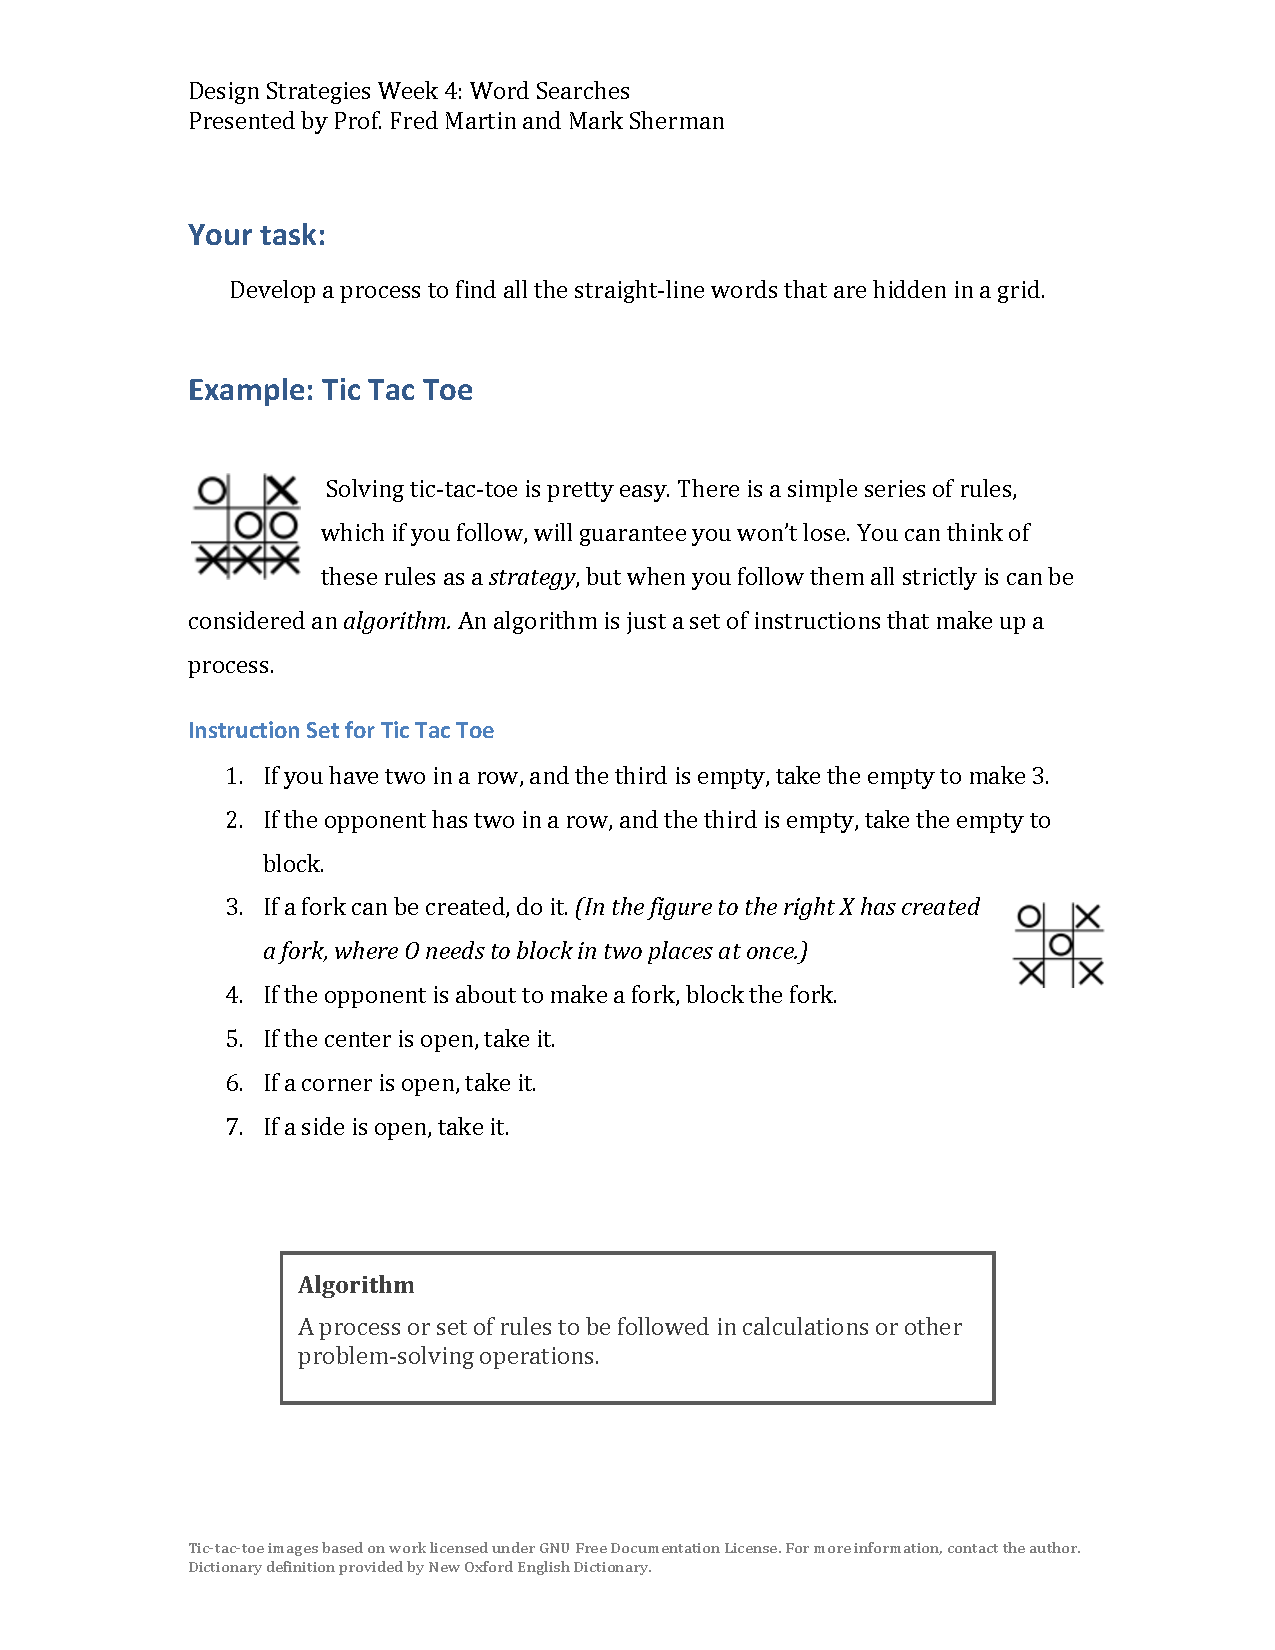
\includegraphics[width=\textwidth]{appendix/word_search_worksheet1.pdf} 
   \caption{First page of the worksheet given to the students during the Word Search activity. This worksheet explains algorithms through the explanation of tic-tac-toe.}
   \label{fig:StudentWorksheet1}
\end{figure}
	
\begin{figure}%  figure placement: here, top, bottom, or page
   \centering
   %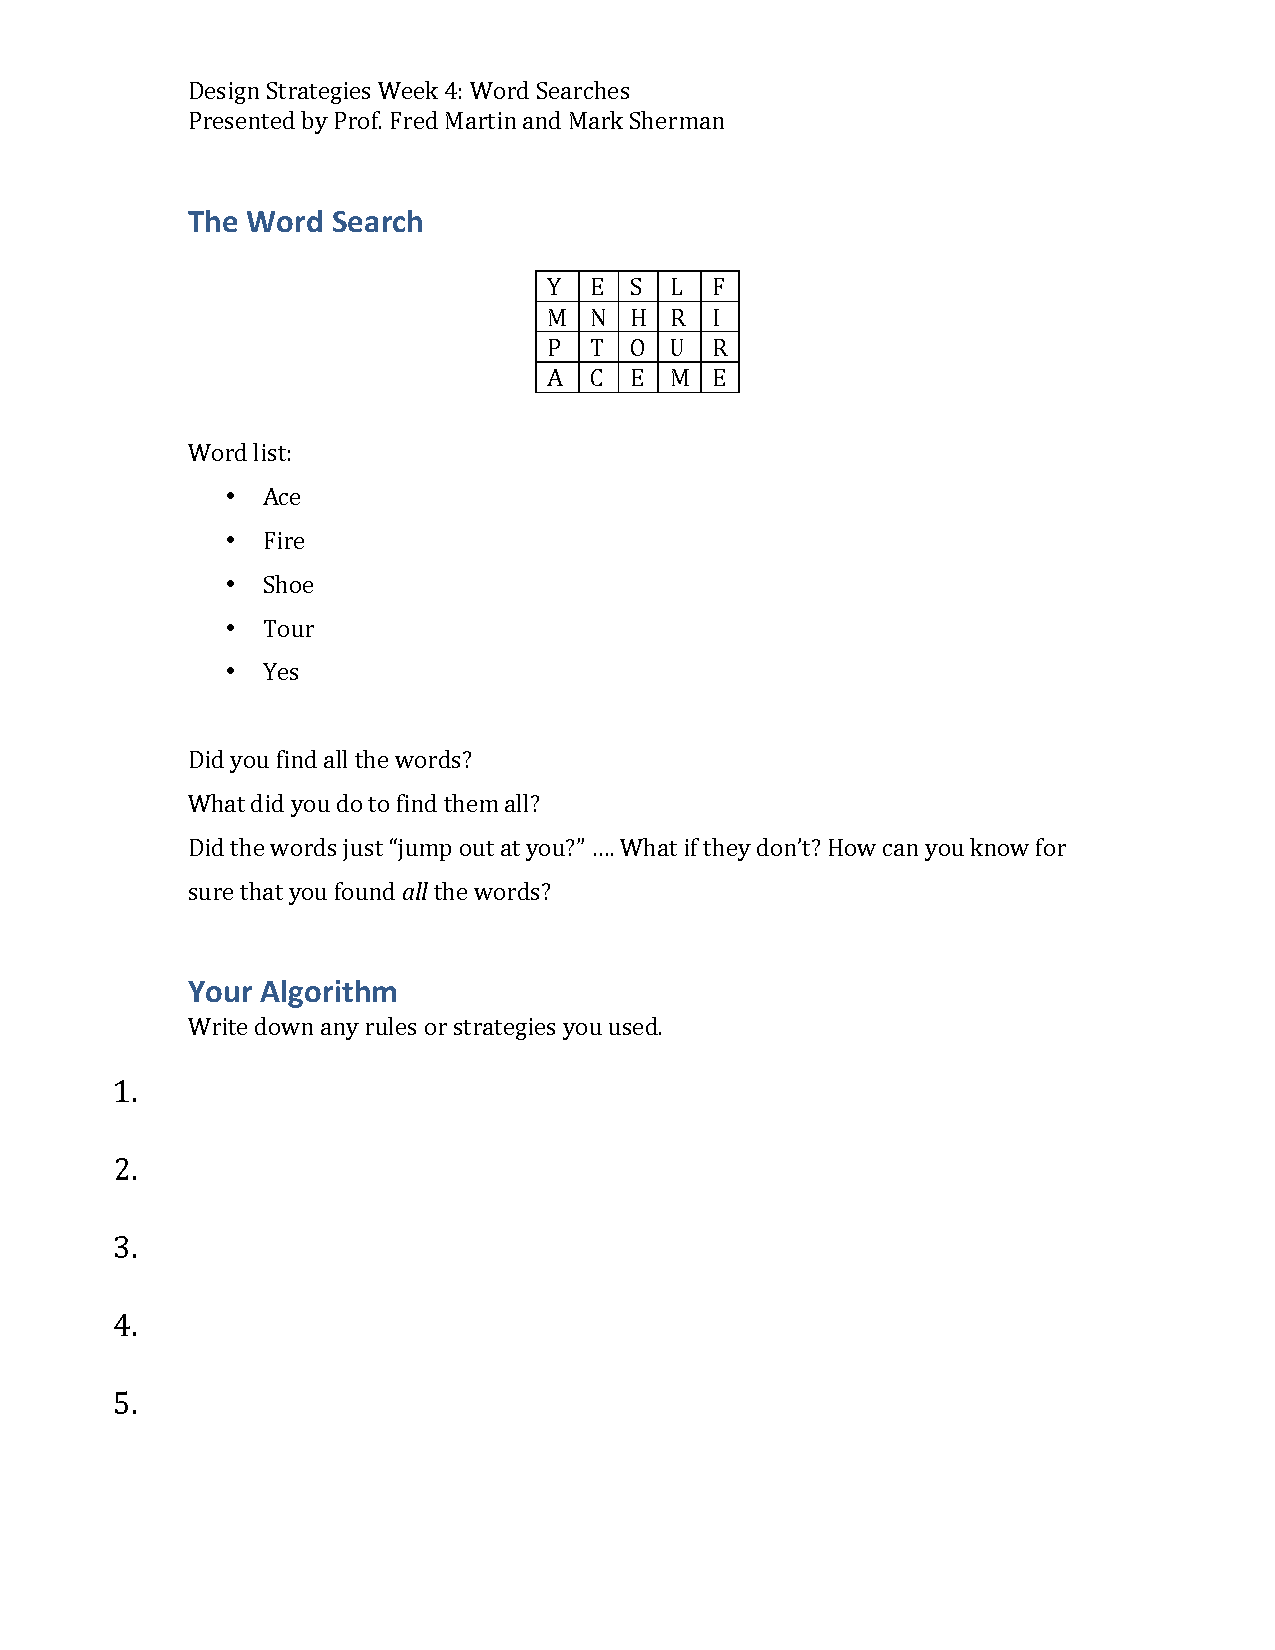
\includegraphics[width=\textwidth]{appendix/word_search_worksheet2.pdf} 
   \caption{Second page of the worksheet given to the students during the Word Search activity. This sheet guided the student through the creation of an example algorithm.}
   \label{fig:StudentWorksheet2}
\end{figure}
	
\begin{figure}%  figure placement: here, top, bottom, or page
   \centering
   %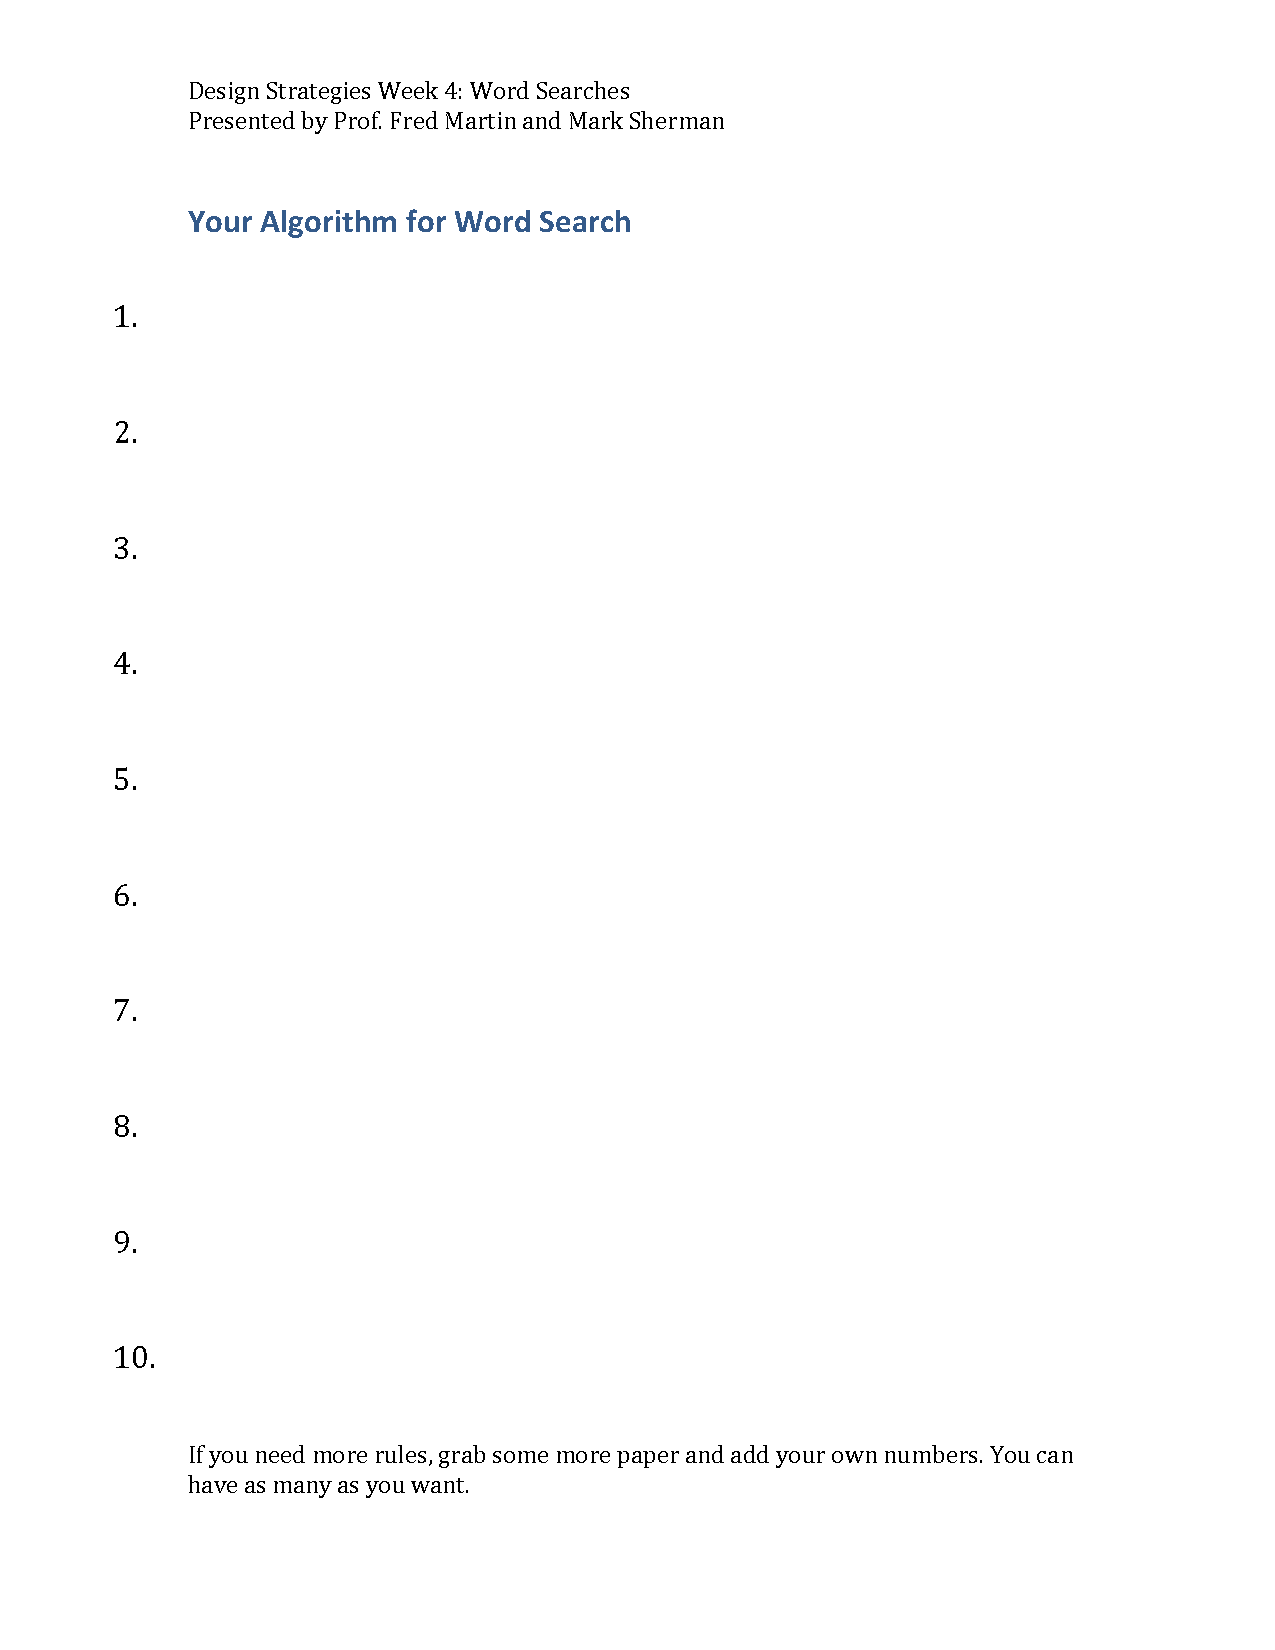
\includegraphics[width=\textwidth]{appendix/word_search_worksheet3.pdf} 
   \caption{Third page of the worksheet given to the students during the Word Search activity. This sheet provided space for students to design their algorithm.}
   \label{fig:StudentWorksheet3}
\end{figure}

%\section{Word Search Puzzle}
	\label{sec:wordsearchpuzzle}
	Figure \ref{fig:wordsearch-puzzle} is one of the two puzzles given to the students. Solutions have been highlighted.
	
	%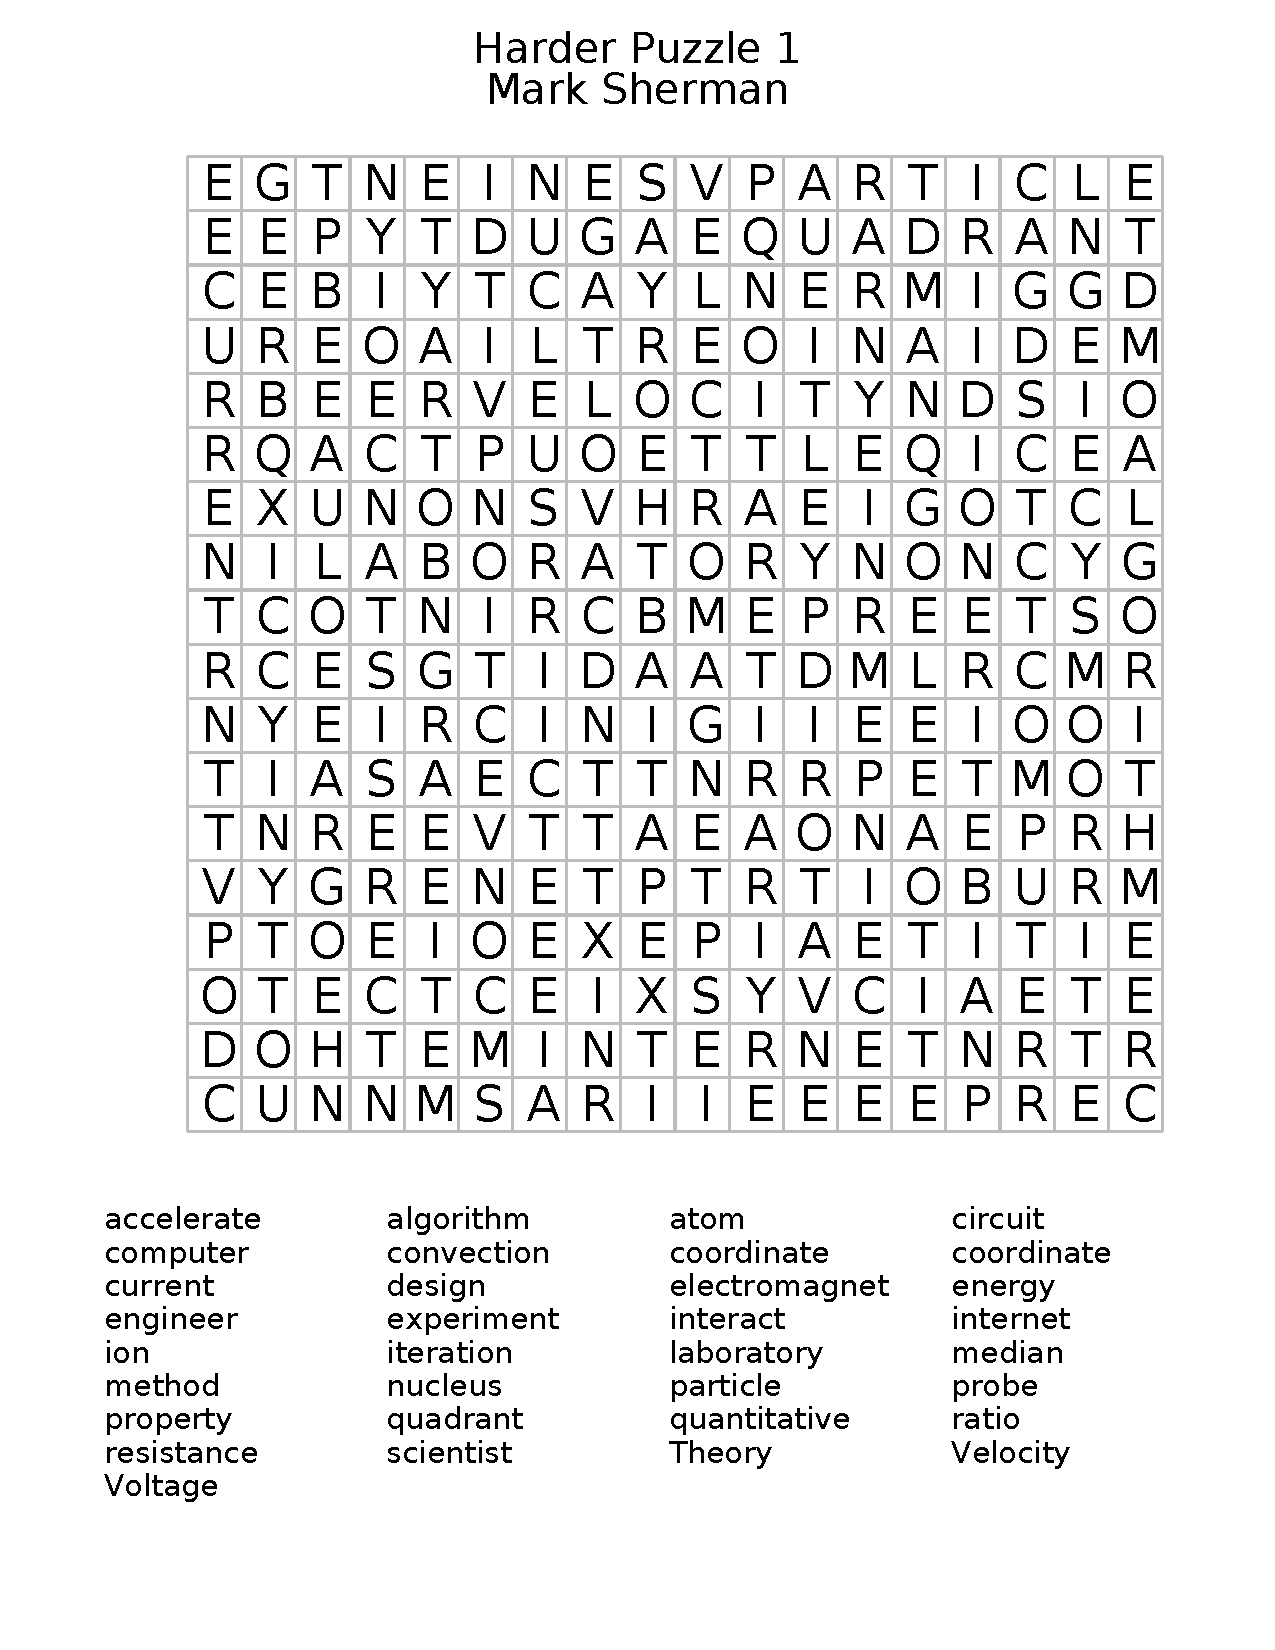
\includepdf[pages=-]{appendix/word_search_puzzle1.pdf}
	%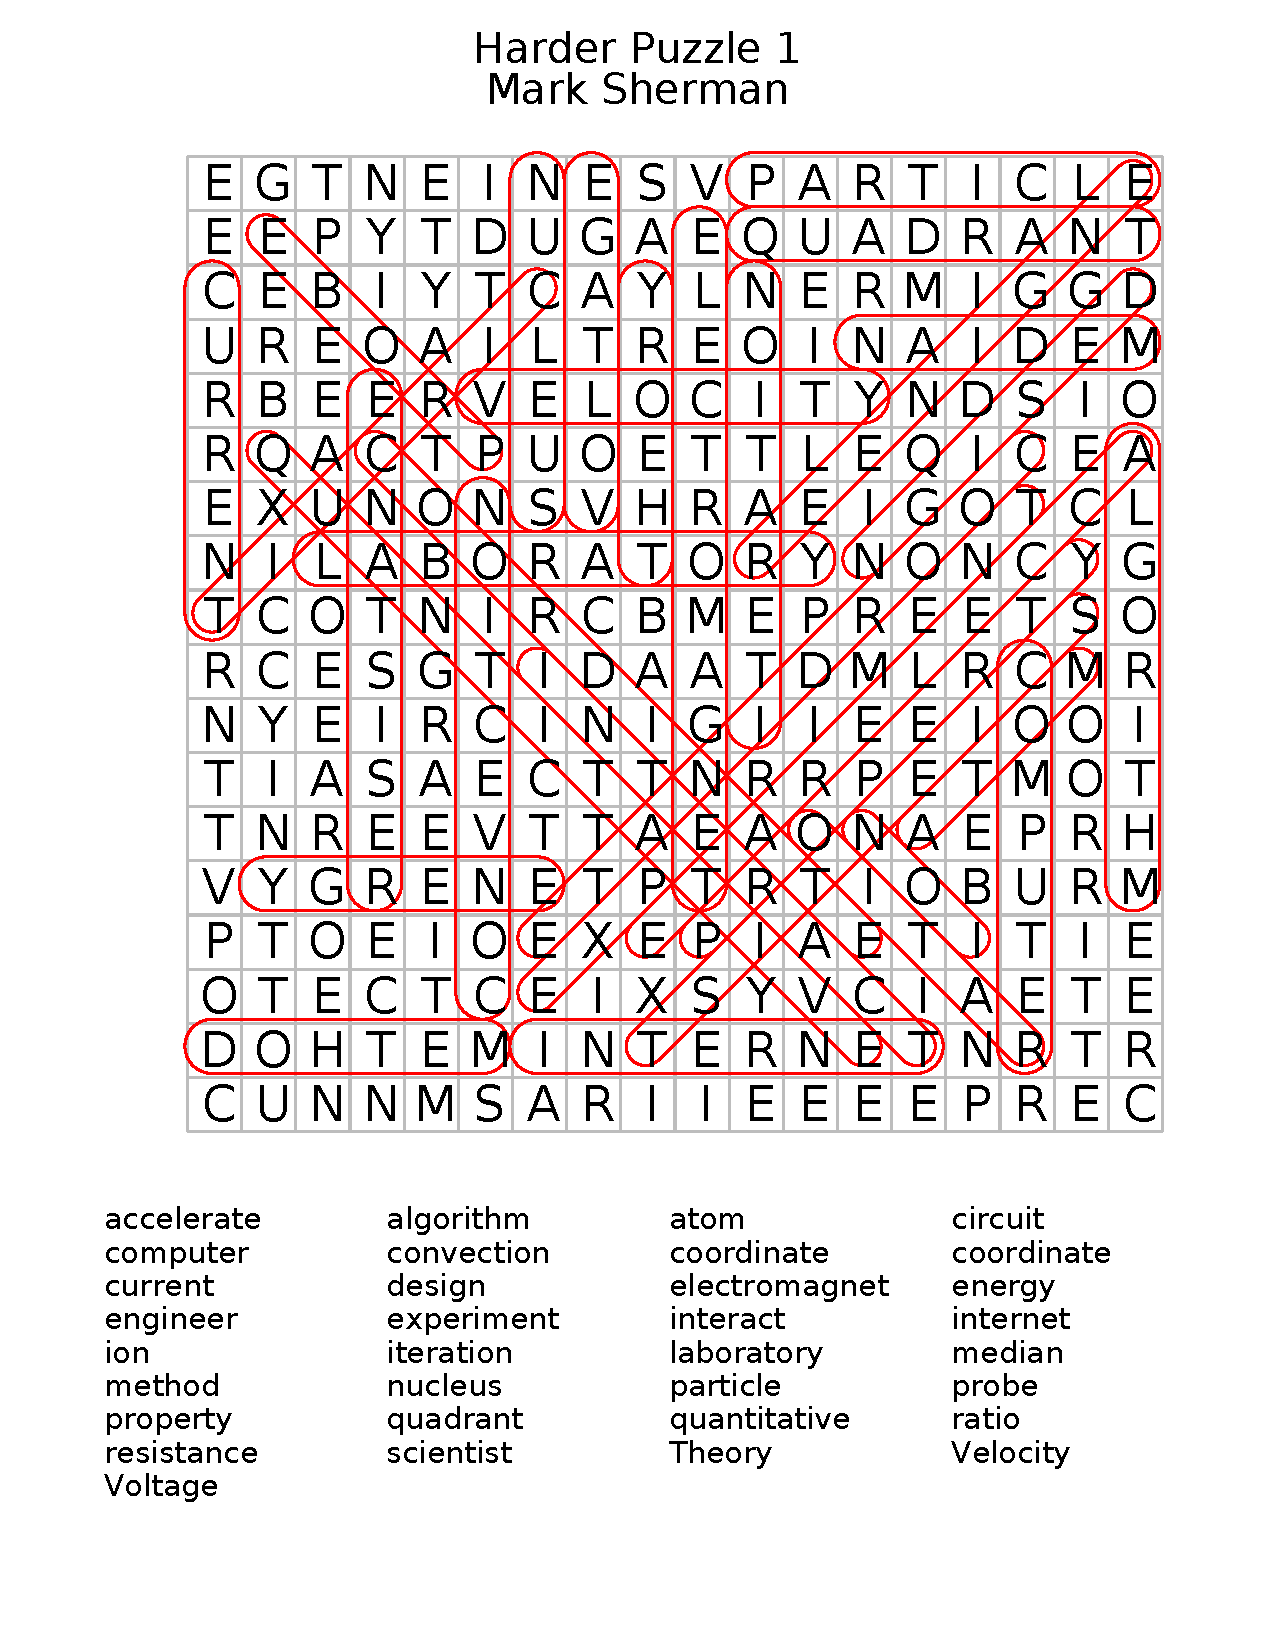
\includepdf[pages=-]{appendix/word_search_puzzle1key.pdf}
	
	\begin{figure}%  figure placement: here, top, bottom, or page
   	\centering
   	%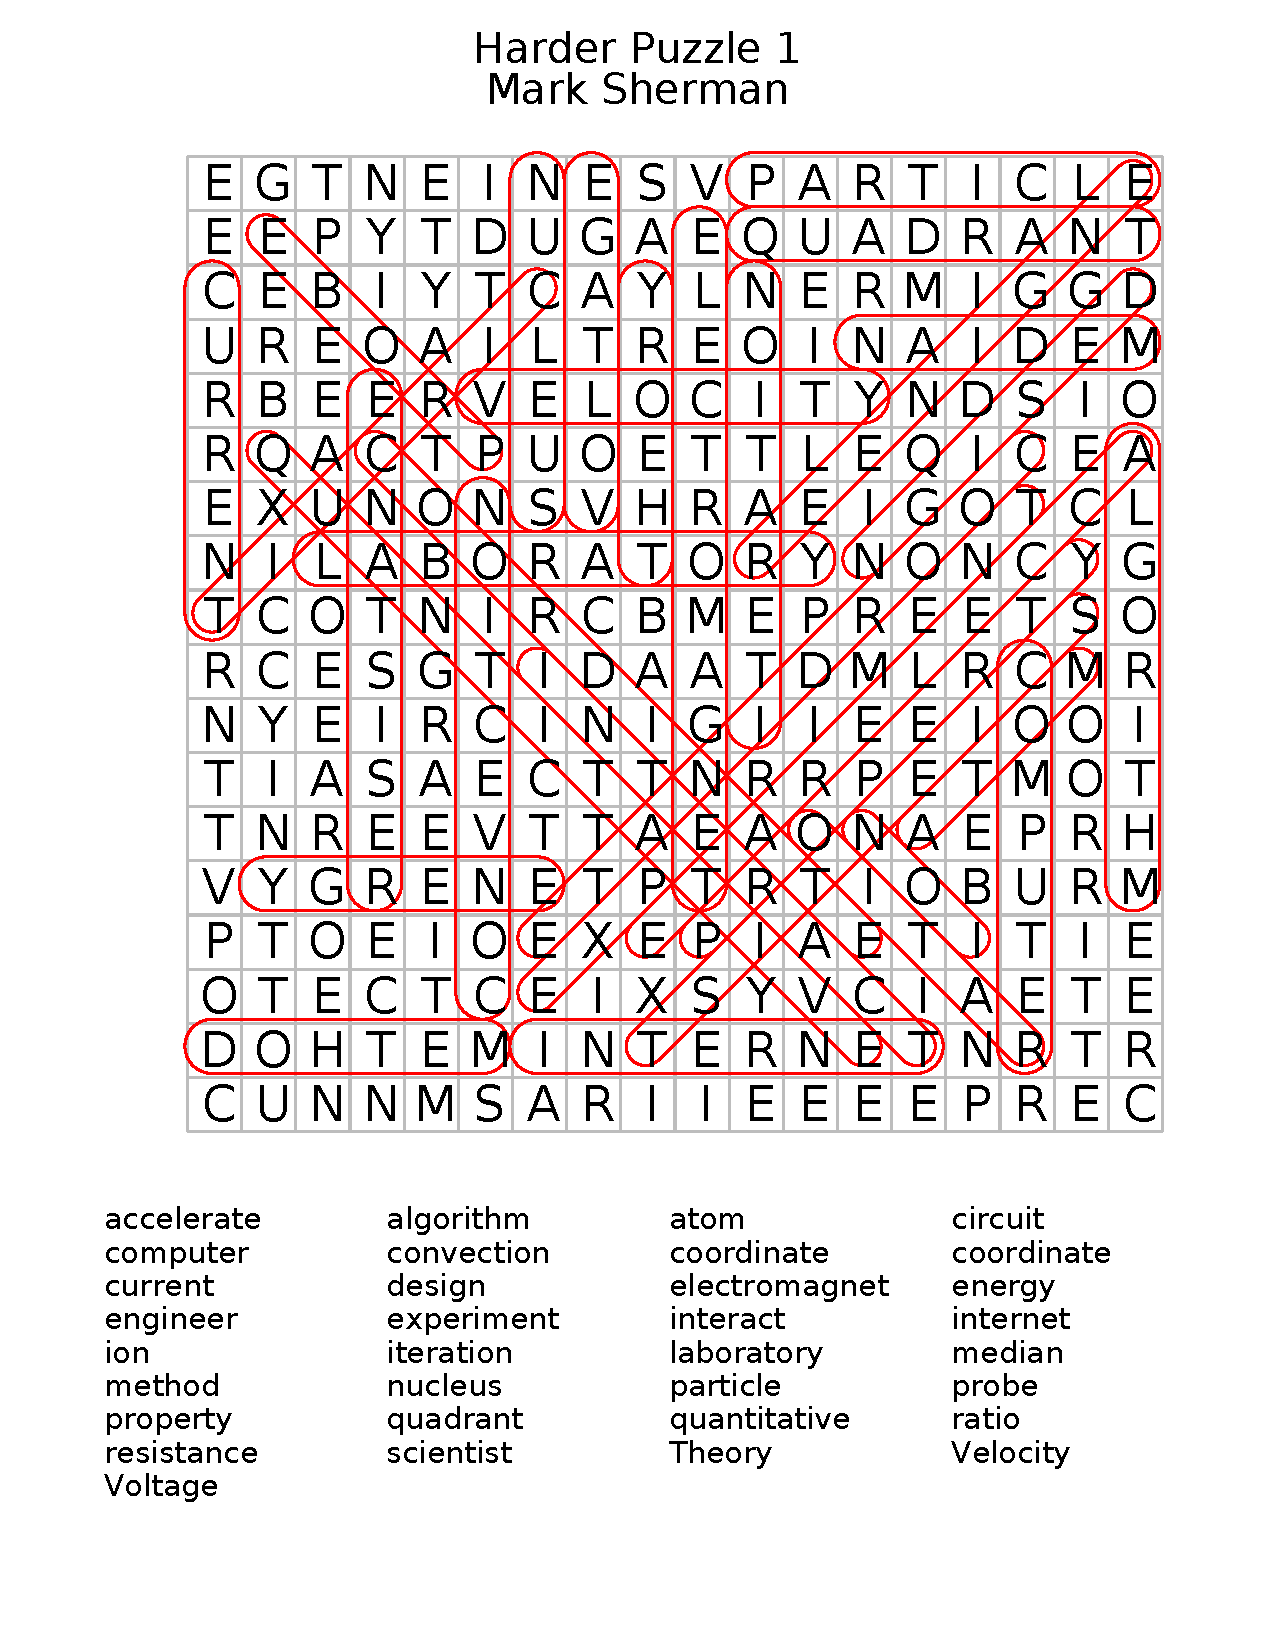
\includegraphics[width=\textwidth]{appendix/word_search_puzzle1key.pdf} 
   	\caption{Word search puzzle provided to the students. The hidden words are shown.}
   	\label{fig:wordsearch-puzzle}
	\end{figure}
	


%\section{Elevator Control Activity Instructions}

	\label{sec:elevator_handout}
	Figure \ref{fig:elevator-instructions} shows the instruction sheet that was given to students at the beginning of the Elevator Control Activity.
	%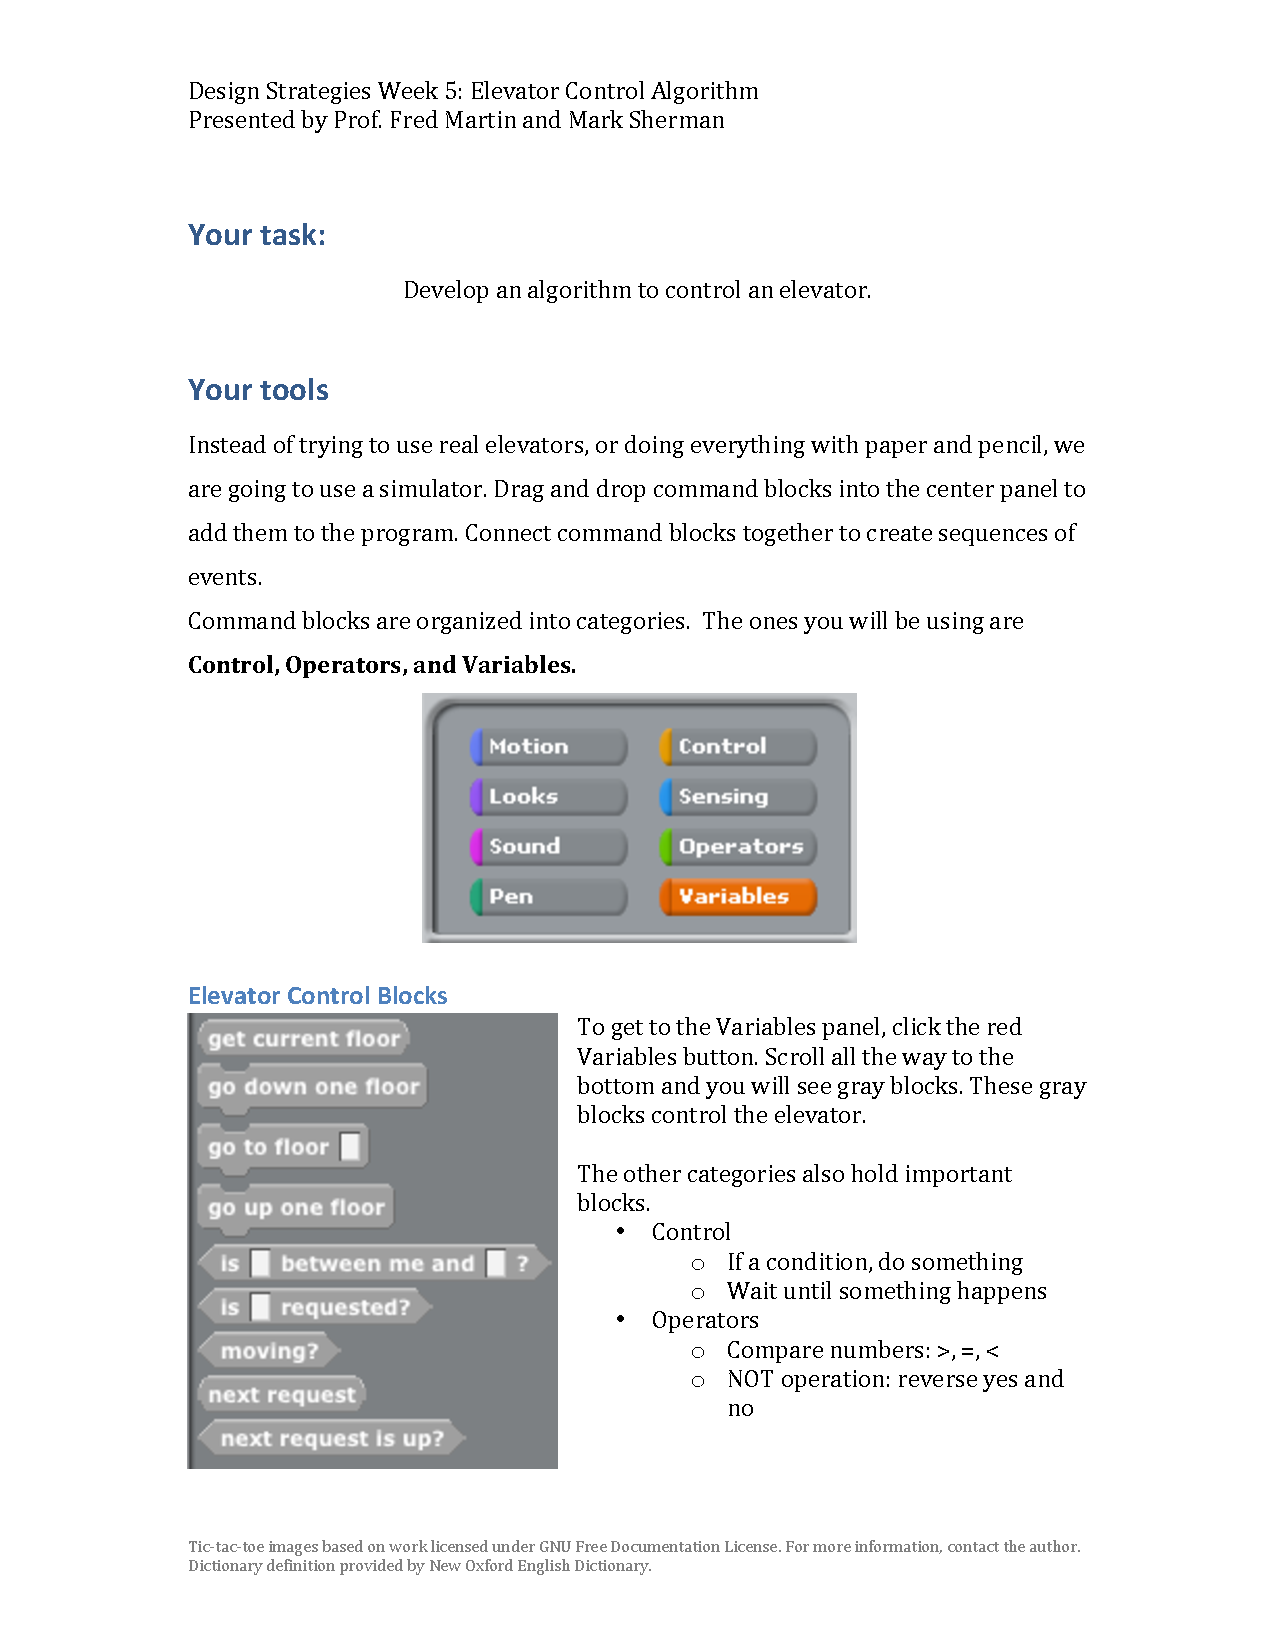
\includepdf[pages=-]{appendix/elevator_instructions.pdf}
	
	\begin{figure}%  figure placement: here, top, bottom, or page
   	\centering
   	%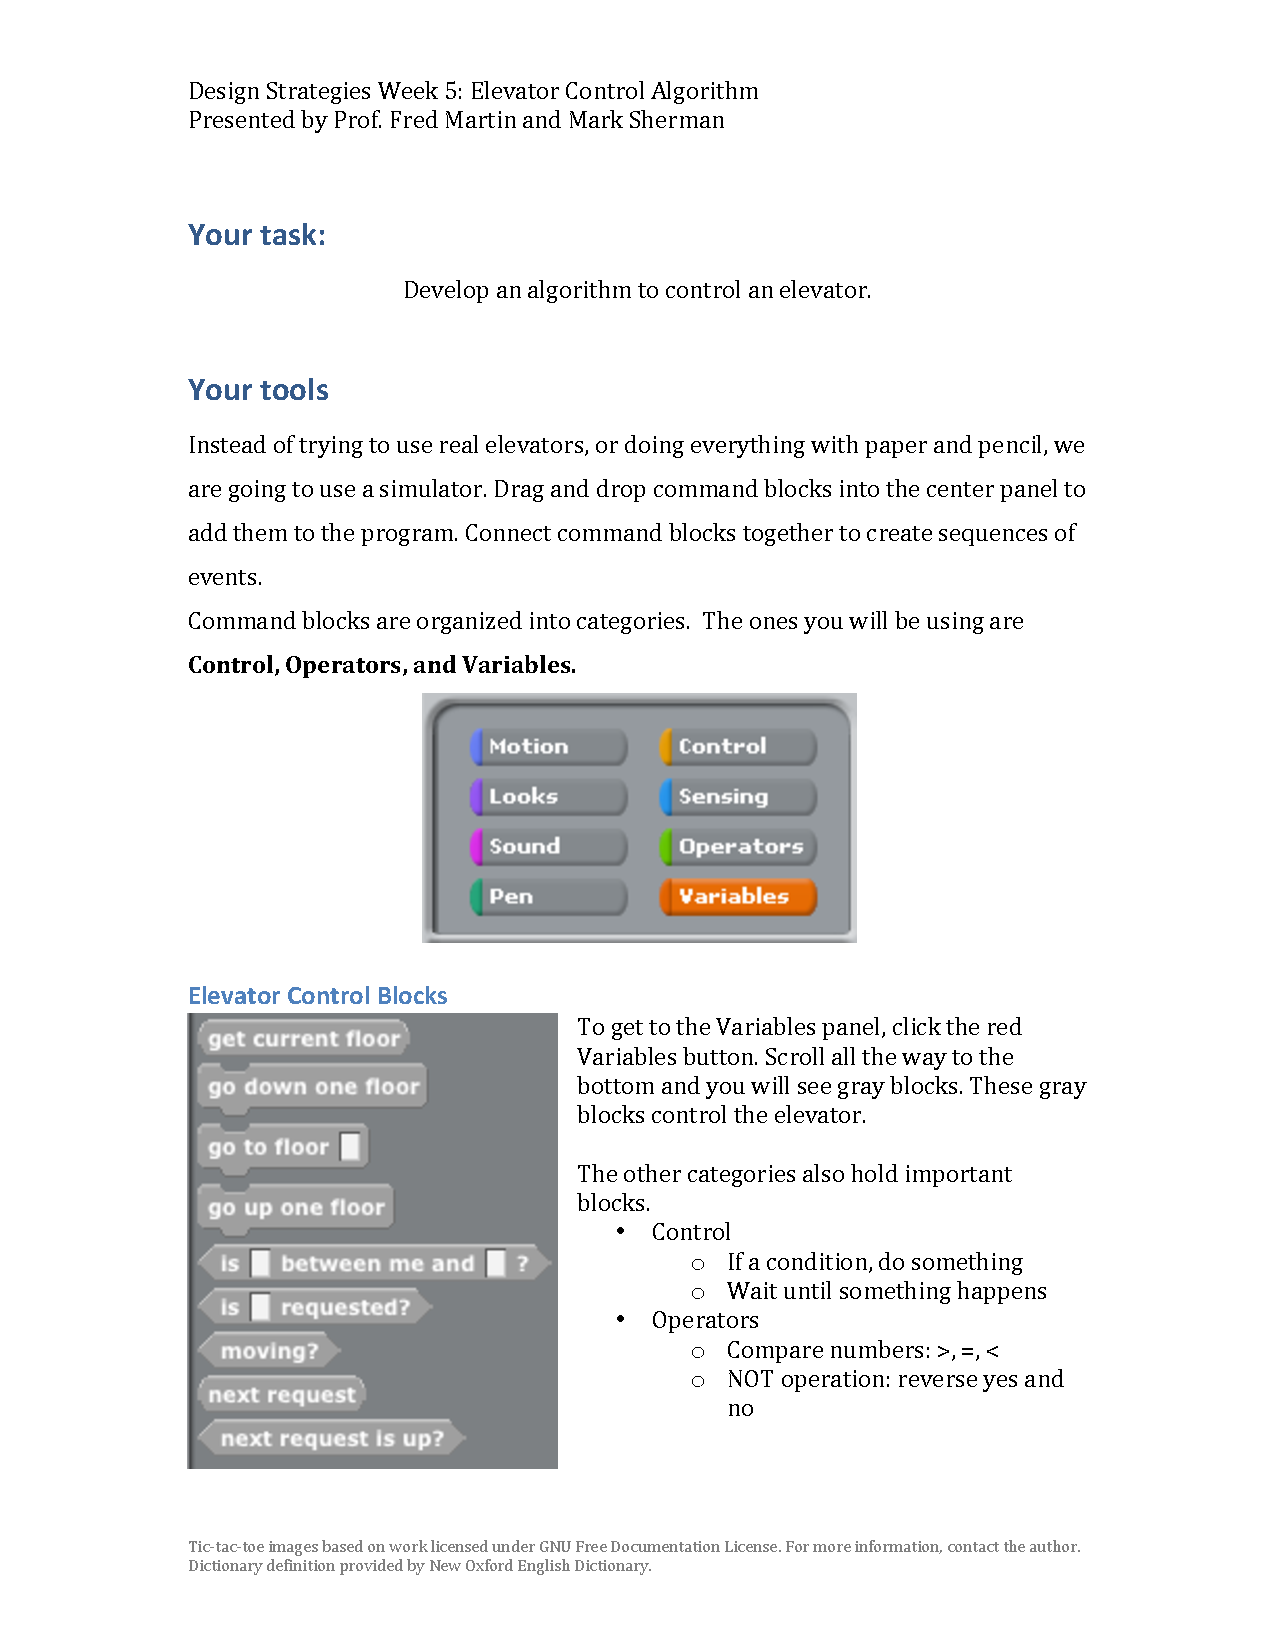
\includegraphics[width=\textwidth]{appendix/elevator_instructions.pdf} 
   	\caption{Elevator Control instruction sheet.}
   	\label{fig:elevator-instructions}
	\end{figure}


\chapter{IRB Compliance Documents}


\section{Parent Consent Form}  \label{sec:parent_consent}
	Figures \ref{fig:consent1} and \ref{fig:consent2} are the Parental Consent Form completed by the legal guardians of all participants in the study. This form was also available in Spanish.
	
	%TODO This form provides identifying information (the YDO/Howard). Should it be included? Censored?

	%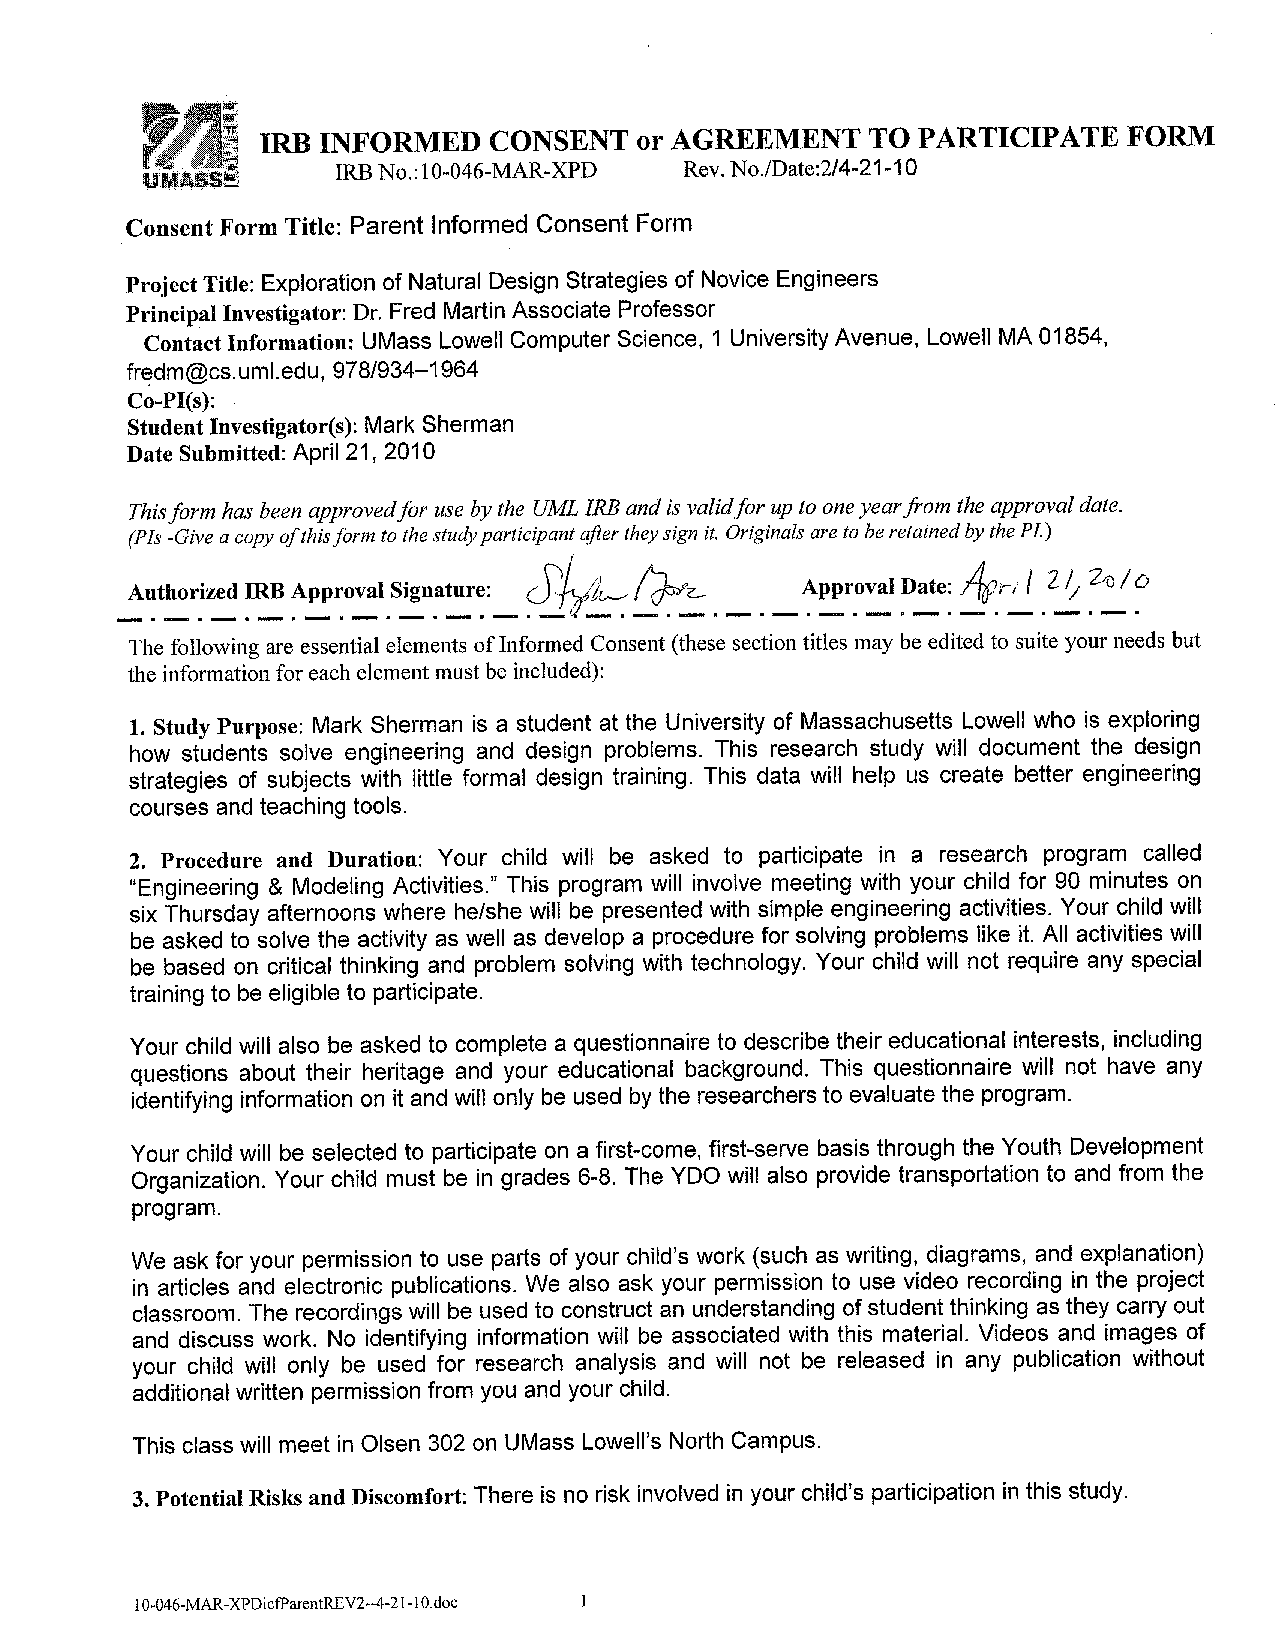
\includepdf[pages=-]{appendix/irb_parent_consent.pdf}
	
	\begin{figure}%  figure placement: here, top, bottom, or page
   	\centering
   	%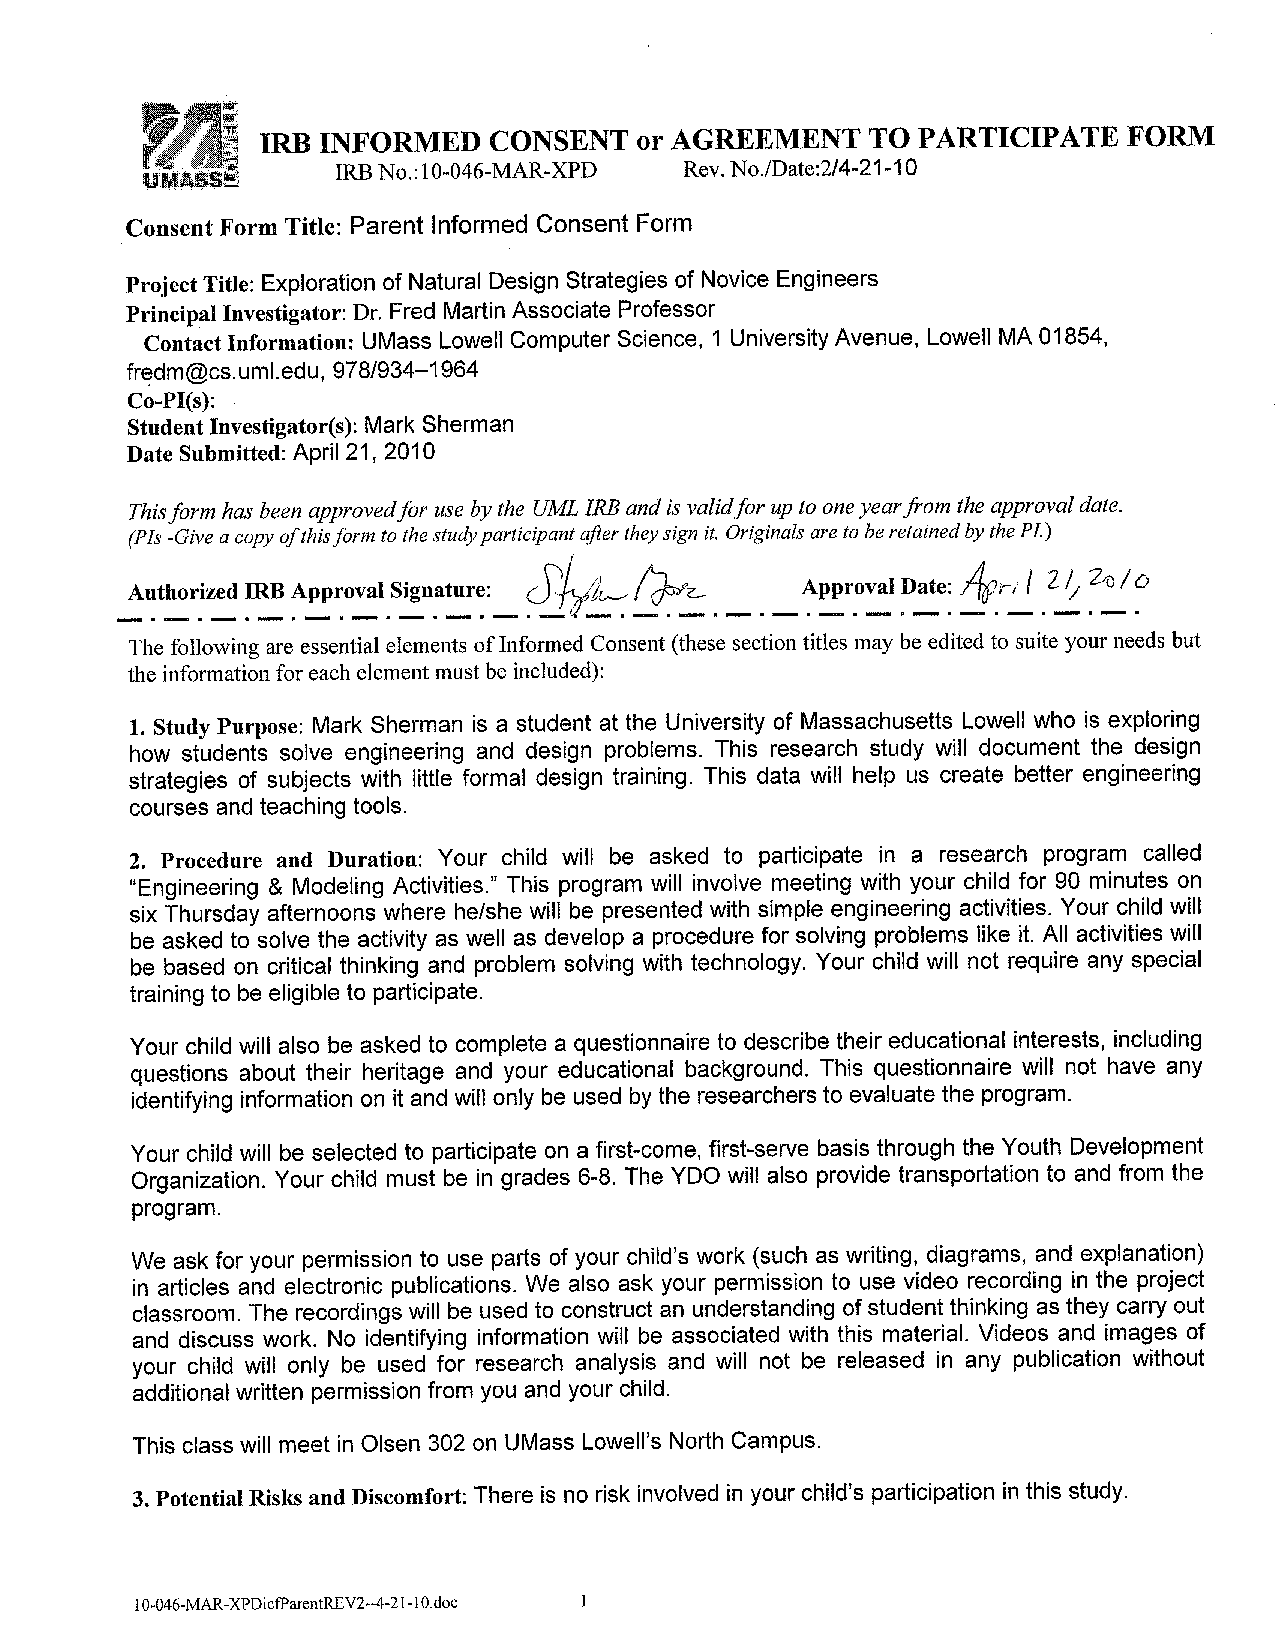
\includegraphics[width=\textwidth]{appendix/irb_parent_consent.pdf} 
   	\caption{Parental consent form, page 1.}
   	\label{fig:consent1}
	\end{figure}

	\begin{figure}%  figure placement: here, top, bottom, or page
   	\centering
   	%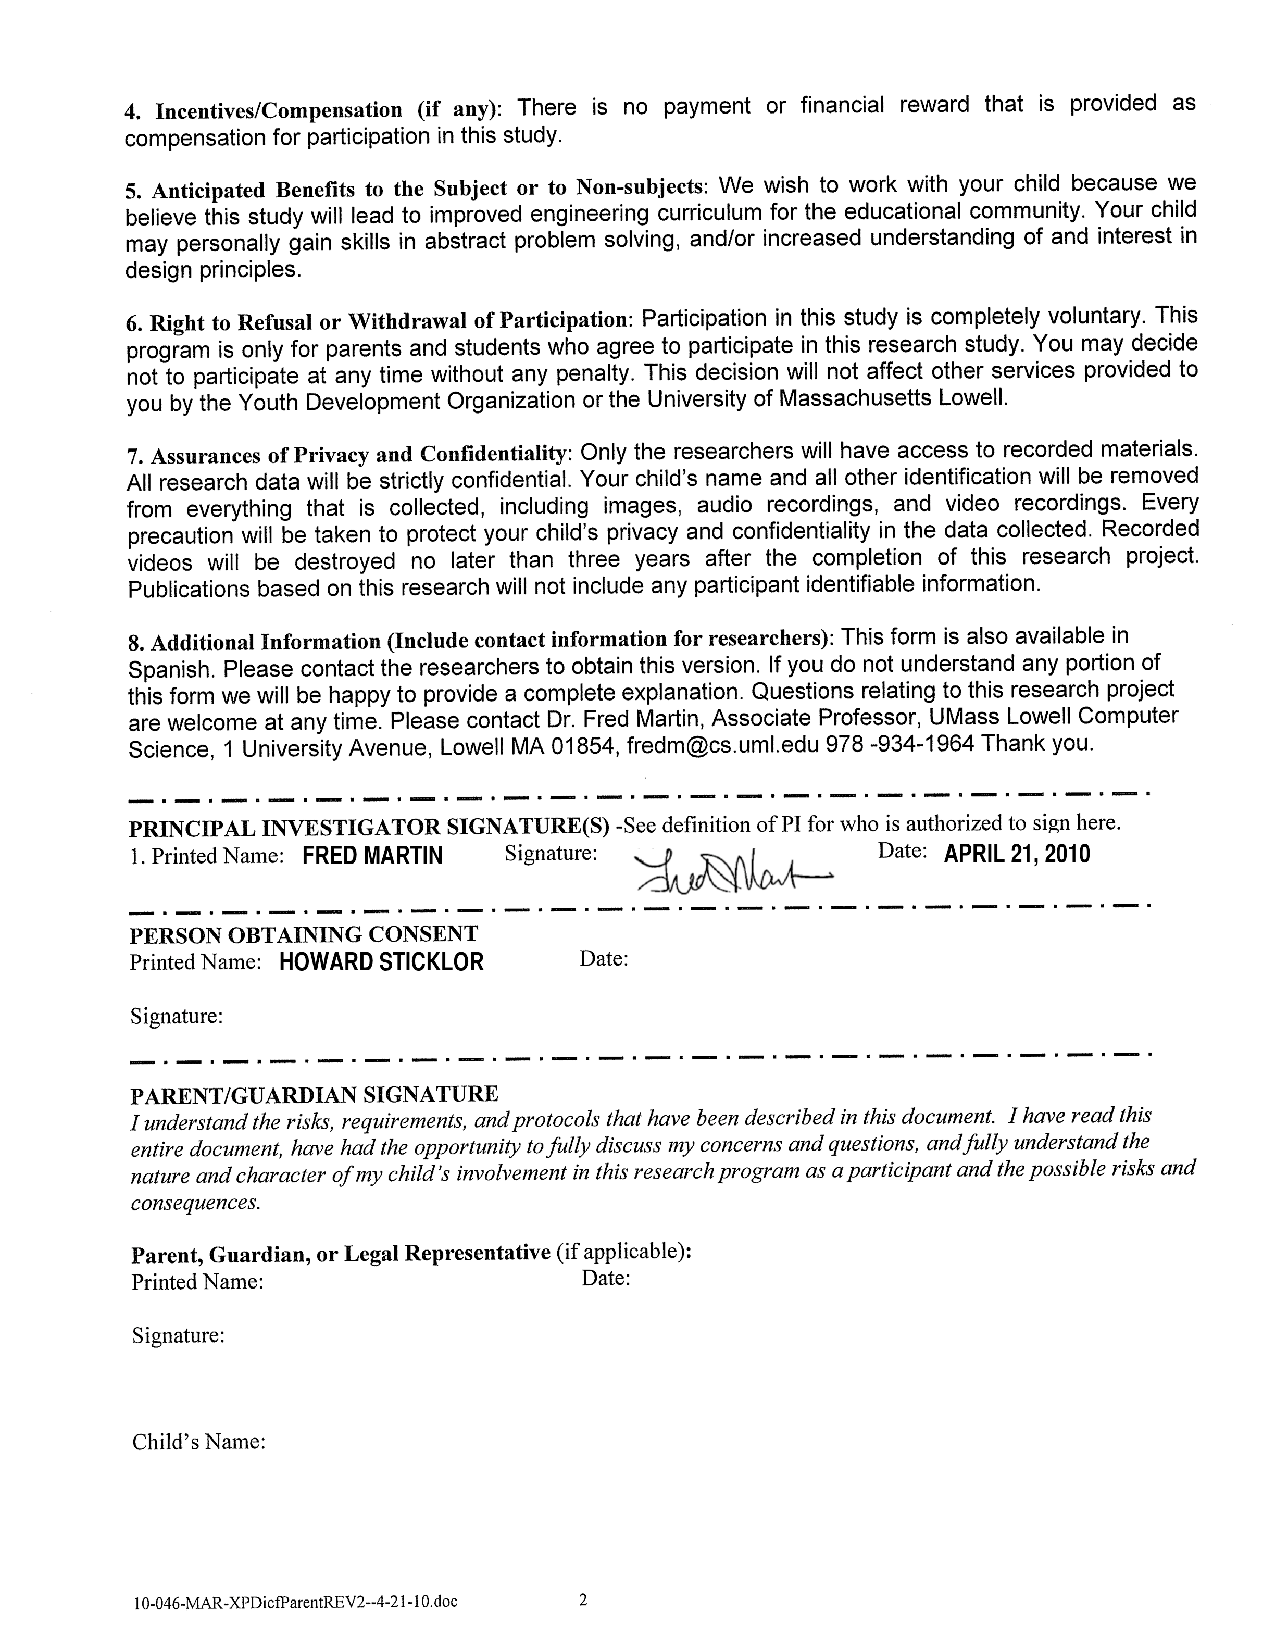
\includegraphics[width=\textwidth]{appendix/irb_parent_consent2.pdf} 
   	\caption{Parental consent form, page 2.}
   	\label{fig:consent2}
	\end{figure}

\section{Student Assent Form} \label{sec:student_assent}
	
	Figures \ref{fig:assent1} and \ref{fig:assent2} are the Student Assent Form completed by all of the participants in the study. 

	%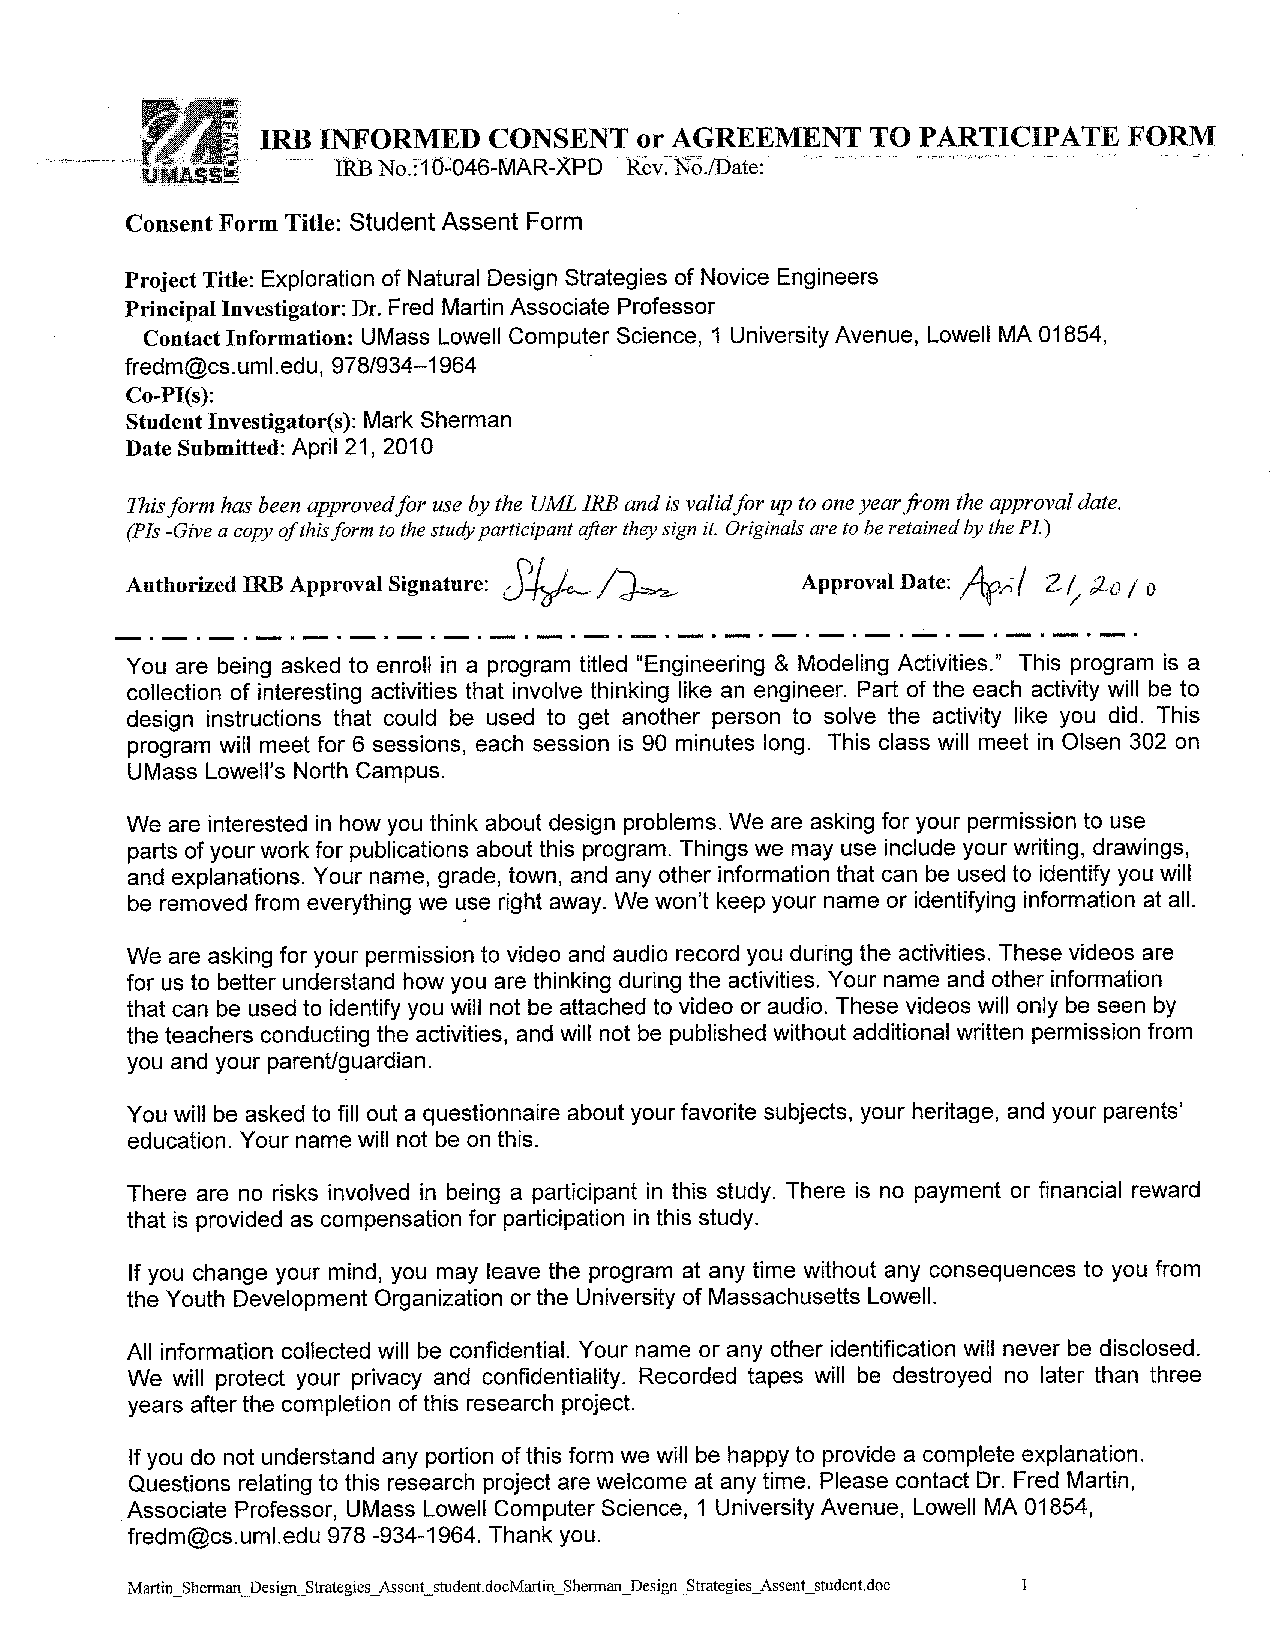
\includepdf[pages=-]{appendix/irb_student_assent.pdf}
	
	\begin{figure}%  figure placement: here, top, bottom, or page
   	\centering
   	%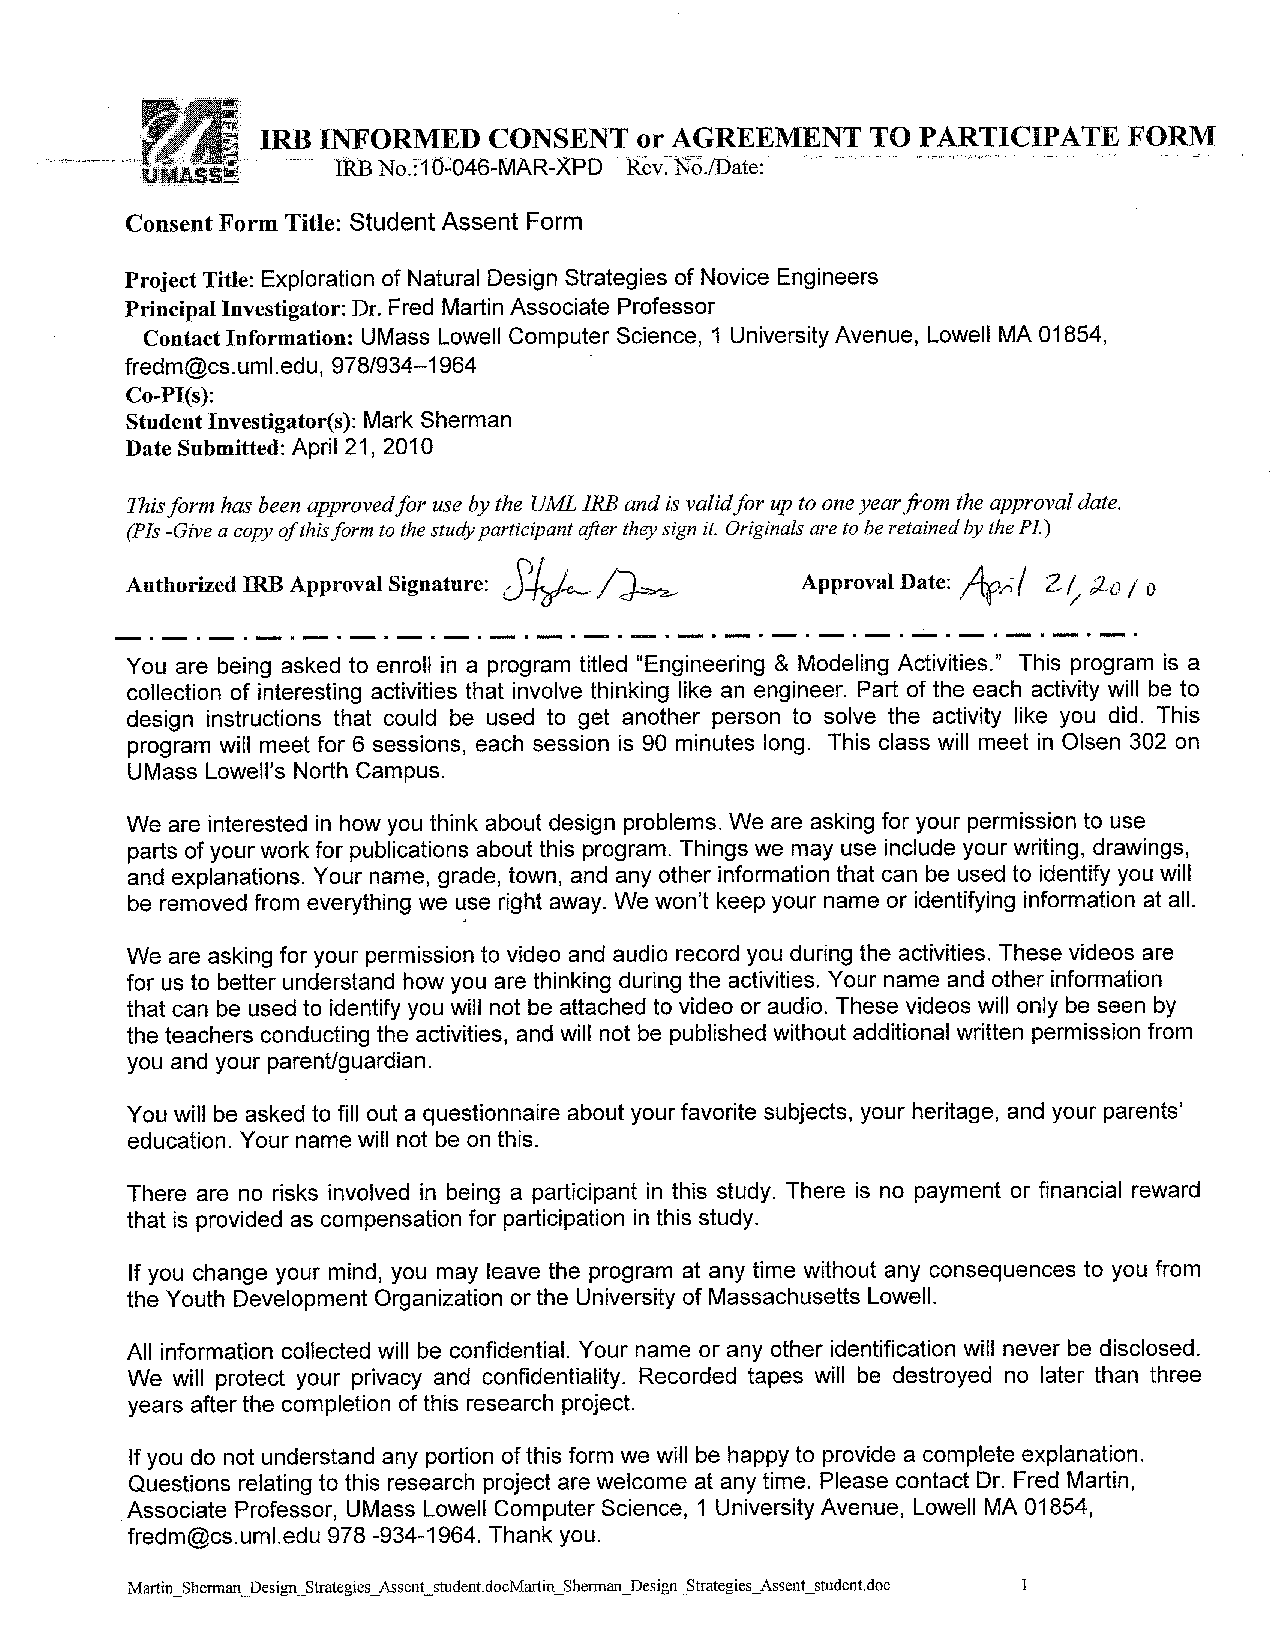
\includegraphics[width=\textwidth]{appendix/irb_student_assent.pdf} 
   	\caption{Student assent form, page 1.}
   	\label{fig:assent1}
	\end{figure}
	
	\begin{figure}%  figure placement: here, top, bottom, or page
   	\centering
   	%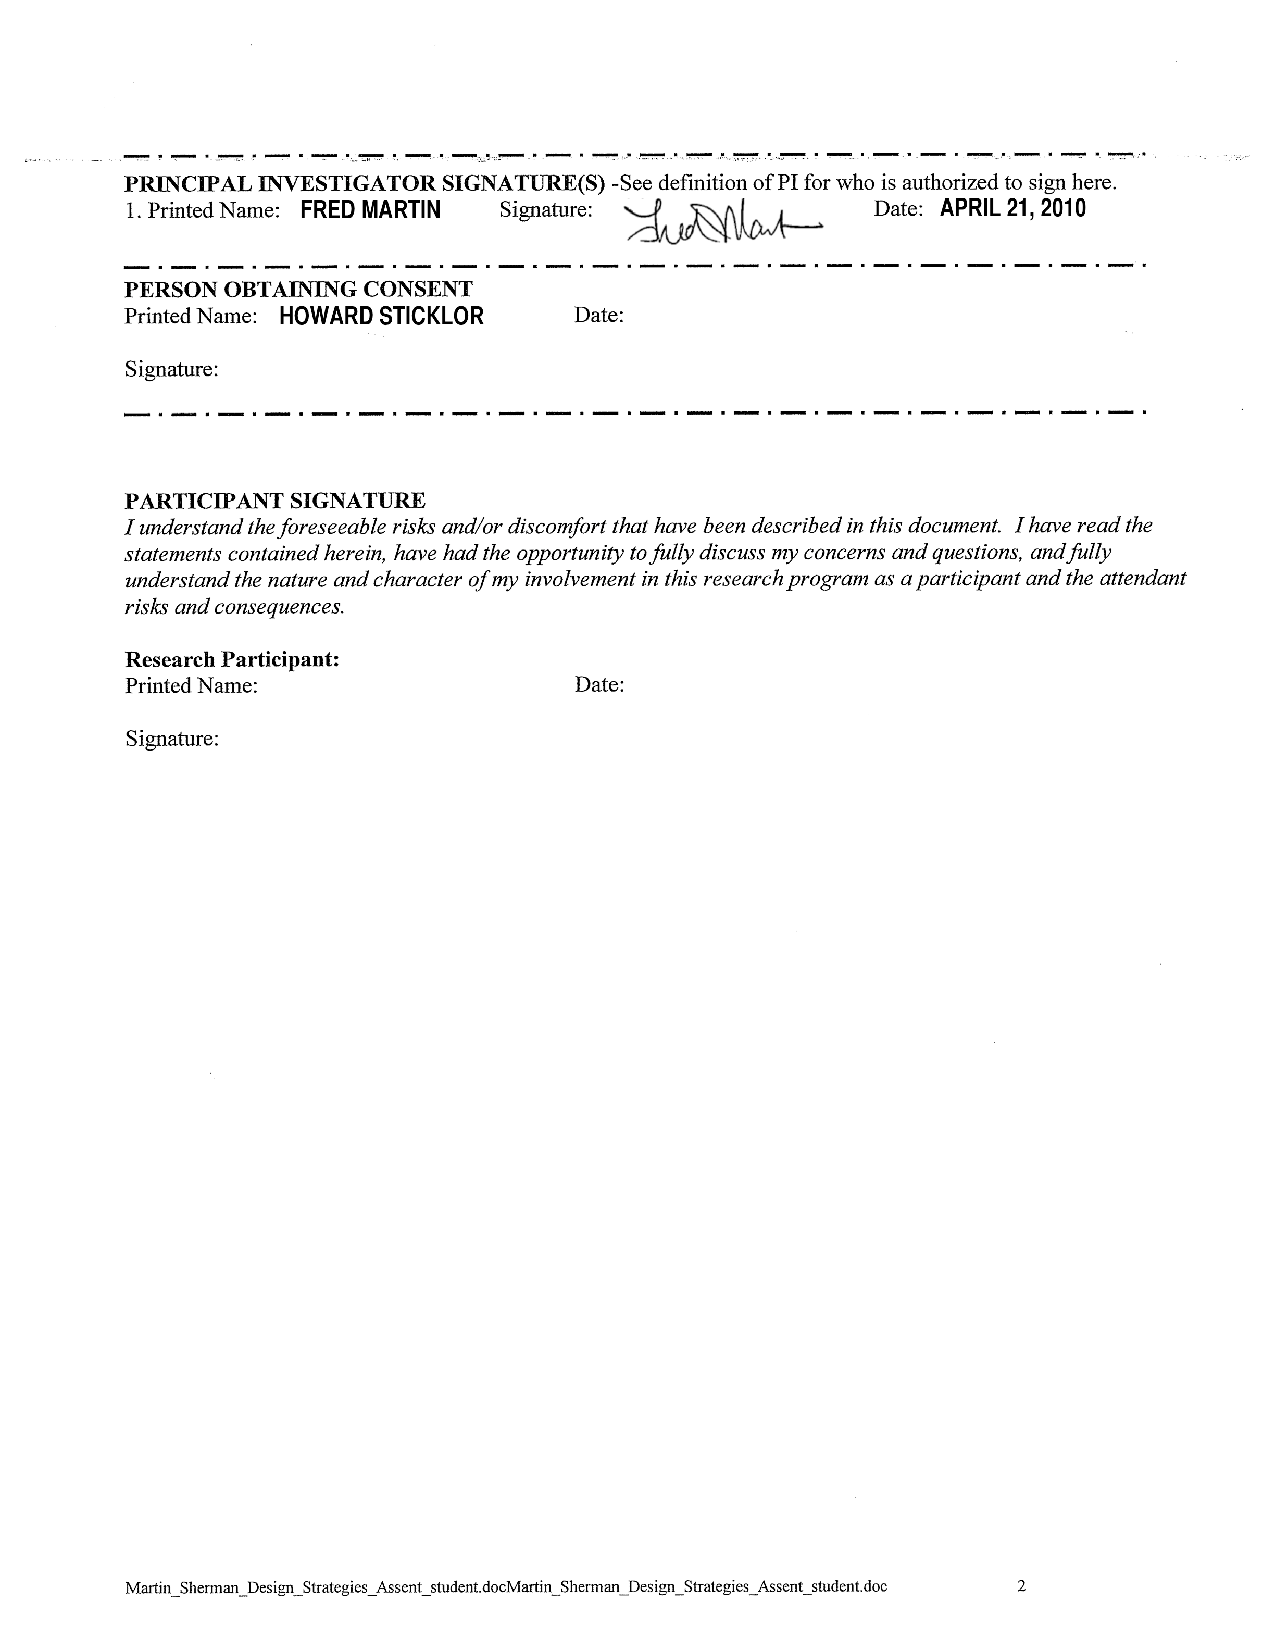
\includegraphics[width=\textwidth]{appendix/irb_student_assent2.pdf} 
   	\caption{Student assent form, page 2.}
   	\label{fig:assent2}
	\end{figure}